\documentclass[slidestop,mathserif,xcolor=dvipsnames]{beamer}
\usepackage[scheme=plain]{ctex}

\usepackage{beamerthemesplit}
\usepackage{color}
\usepackage{soul}
\usepackage{xspace}
\usepackage{pdfpages}
\usepackage{epic}
\usepackage{graphicx}
\usepackage{qrcode}
\usepackage{geometry}
\usepackage{curves}
\usepackage{amsmath,amssymb}
%\usepackage[latin1]{inputenc}
\usepackage{colortbl}
\usepackage[english]{babel}
\usepackage{url}
\usepackage{pgf,pgfarrows,pgfnodes,pgfautomata,pgfheaps,pgfshade}
\usepackage{eqlist}
\usepackage{multirow}
\usepackage{alltt}
\usepackage{extarrows}
\usepackage{pgfplots}
\usepackage{pgfplotstable}
\usepackage{subfigure}
\usepackage{extarrows}
\usepackage{boxedminipage}
\usepackage{booktabs}
\usepackage{algorithm2e}
\usepackage{algorithmic}

\usepackage{lipsum}
\newcommand\blfootnote[1]{%
  \begingroup
  \renewcommand\thefootnote{}\footnote{#1}%
  \addtocounter{footnote}{-1}%
  \endgroup
}

\usepackage{tikz}
\usepackage{makecell}
\usetikzlibrary{patterns}

\definecolor{darkblue}{rgb}{0,0,0.5}
\definecolor{darkgreen}{rgb}{0,0.6,0}
\definecolor{mymagenta}{RGB}{238,0,238}
\newcommand{\blue}[1]{\textcolor{blue}{#1}}
\newcommand{\red}[1]{\textcolor{red}{#1}}
\newcommand{\dgreen}[1]{\textcolor{darkgreen}{#1}}
\newtheorem*{mybox}{}
\newcommand{\dist}{\mathrm{dist}}
\newcommand{\sss}[1]{{\scriptscriptstyle{#1}}}
\newcommand{\nb}{\textbf{N.B.}}
\newcommand{\base}{{\text{b}}}
\newcommand{\opt}{{\text{o}}}
\newcommand{\tr}{\text{tr}}
\newcommand{\drop}{\text{drop}}
\newcommand{\geo}{\text{geo}}



\usetheme{Madrid} % Beamer theme v 3.0

\usecolortheme[RGB={20, 40, 80}]{structure} % Beamer color theme

%\useoutertheme{shadow}
\setbeamertemplate{frametitle}{%
\begin{beamercolorbox}[wd=\paperwidth, ht=0.5cm, dp=0.2cm]{frametitle}
    \hspace*{2mm}\usebeamerfont{frametitle}\insertframetitle
\end{beamercolorbox}
}
\useoutertheme{shadow} % If this command is called after \setbeamertemplate,
% then there is no white space on the top of the page.

\newcommand\SP{\mathcal{S}}
\newcommand\XX{{\mathcal{X}}}
\newcommand\RR{{\mathbb{R}}}
\newcommand\NN{{\mathbb{N}}}
\newcommand\ZZ{{\mathbb{Z}}}
\newcommand\QQ{{\mathbb{Q}}}
\newcommand\poll{{\sc poll }}
\newcommand\search{{\sc search }}
\newcommand\cuter{{\sf CUTEr }}
\newcommand\MADS{{\sc mads }}
\newcommand\PPP{\mathcal{P}}
\newcommand\OOO{{\mathcal{O}}}
\newcommand\dfo{\texttt{DFO}}
\newcommand\newuoas{NEWUOAs\xspace}
\newcommand\newuoa{\texttt{NEWUOA}}
\newcommand\ssd{\texttt{SSD}}
\newcommand\etal{\textit{et al.}}
%\newcommand\st{\textnormal{s.t.}}

\newcommand{\bphi}{\bar{\phi}}

\newcommand{\qua}{q}%a função quadratica
\newcommand{\quaa}{q}%a função quadratica no Cap2
\newcommand{\fo}{f}%a função objectivo
\newcommand{\frau}{g}%a função que se usa no 4.1.
\newcommand{\drau}{\mathcal{D}}%o dominio das funções que se usam no 4.1. e por aí a diante
\newcommand{\vad}{u}%as variaveis em R^n
\newcommand{\pon}{w}%os pontos em R^n
\newcommand{\Pon}{W}%o conjunto dos pontos em R^n
\newcommand{\coe}{\alpha}%os coeficientes no Cap4
\newcommand{\tay}{T}%a aproximação de taylor
\newcommand{\dimqua}{\frac{(n+1)(n+2)}2}%dimensão do espaço das quadraticas em R^n
\newcommand{\dimquah}{(n+1)(n+2)/2}%dimensão do espaço das quadraticas em R^n horizontal
\newcommand{\nstep}{k}%a aproximação de taylor
\newcommand{\azul}{\textcolor{blue}}
\def\real{\mathbb{R}}

\def\boite{\hfill{$\hbox{\vrule height4pt width4pt}$}}
\def\demo{\noindent{\sc Proof: \ }}
\newtheorem{Axm}{Axiom}
\newtheorem{Def}{Definition}
\newtheorem{Alg}{Algorithm}
\newtheorem{Lem}[Def]{Lemma}
\newtheorem{Ass}{Assumption}
\newtheorem{Prop}[Def]{Proposition}
\newtheorem{Th}[Def]{Theorem}
\newtheorem{Cor}[Def]{Corollary}
\newtheorem{Res}[Def]{Result}
\newtheorem{Ex}[Def]{Exemple}
\newtheorem{Hyp}[Def]{Hypothesis}
\newtheorem{Que}[Def]{Question}
\newtheorem{Ans}[Def]{Answer}
\newtheorem{Exer}{Exercise}
\newtheorem{CO}{Necessary optimality condition}
\newtheorem*{BOX}{}
\newtheorem*{PROPT}{Properties of the framework}
\newtheorem*{OBS}{Observasion}
\newtheorem*{GOAL}{Our goal}

\DeclareMathOperator{\Gr}{Gr}
\DeclareMathOperator*{\argmax}{arg\,max}
\DeclareMathOperator*{\argmin}{arg\,min}
\DeclareMathOperator*{\rargmin}{\textcolor{red}{arg\,min}}
\DeclareMathOperator{\aff}{aff}
\DeclareMathOperator{\vol}{vol}
\DeclareMathOperator{\von}{von}
\DeclareMathOperator{\diam}{diam}
\DeclareMathOperator{\gerado}{span}
\DeclareMathOperator{\supp}{supp}
\DeclareMathOperator{\md}{d}

\DeclareMathOperator{\inte}{int}
\DeclareMathOperator{\epi}{epi}


\newtheorem{Fa}[Def]{Simple Fact}

\newtheorem{FOO}{Clarke stationarity}
\DeclareMathOperator{\cm}{cm}
%\newtheorem{CDS}[Def]{A classical direct search algorithm (Coordinate Search)}
\newtheorem{CDS}[Def]{A simple direct search algorithm}

\definecolor{gris}{rgb}{0.6,0.6,0.6}
\definecolor{Maroon2}{rgb}{0.6,0.05,0.03}
\definecolor{Maroon3}{rgb}{0.95,0.9,0.9}
\definecolor{Maroon4}{rgb}{1,0.97,0.97}
\definecolor{Verde}{rgb}{0,0.6019,0.4019}

\definecolor{darkgreen}{rgb}{0,0.6,0}

\setbeamertemplate{footline}
{
\begin{beamercolorbox}{section in head/foot}
%\insertsectionnavigationhorizontal{.5\textwidth}{\hskip0pt plus1filll}{toto}
%\insertsectionnavigationhorizontal{.5\textwidth}{\hskip0pt plus1filll}{tata}
%\insertshortauthor (\insertshortinstitute)  \hspace*{1cm}
\hspace*{2mm}\insertsection
\hfill
\insertframenumber /\inserttotalframenumber \hspace*{2mm}
\end{beamercolorbox}
}

%\setbeamertemplate{itemize/enumerate body begin}{\normalsize}
%\setbeamertemplate{itemize/enumerate subbody begin}{\normalsize}
%\setbeamertemplate{itemize/enumerate subsubbody begin}{\normalsize}

\usenavigationsymbolstemplate

%==============================================================

\hypersetup{
  pdftitle={PDFO},%
  pdfauthor={ZHANG Zaikun},
}

\AtBeginSection[]
{
    \begin{frame}
        \frametitle{Outline}
        \tableofcontents[currentsection]
    \end{frame}
}

\title[\insertsection]
%{PRIMA: Reference Implementation for Powell's Methods with Modernization and Amelioration}
{PRIMA: What, Why, How, and So What?}
\author[]{
  {\href{https://www.zhangzk.net}{Zaikun Zhang}}
  \\[2ex]{\small The Hong Kong Polytechnic University}\\[3ex]
    {
        SIOPT 2023, Seattle
        %\\[3ex]
        \\[9ex]
        %Dedicated to the late Professor \textbf{M. J. D. Powell} FRS (1936--2015)
    }%, PolyU}
    %\\[2ex]
    %\textcolor{darkblue}{In deep memory of late
    %  \href{https://zhangzk.net/powell.html}{Professor M. J. D.  Powell} (1936--2015)}
	}

\date{}

\graphicspath{{./Figs/}}

\let\otp\titlepage

%==============================================================
\setcounter{framenumber}{-1}

\begin{document}

%\maketitle
\begin{frame}[plain]
  \titlepage
%  \begin{center}
%      {\footnotesize Funding: Hong Kong RGC grants 253012/17P, 153054/20P, and 153066/21P.}
%  \end{center}
\end{frame}

\begin{frame}
    \frametitle{What is this talk about?}

    \vspace{10ex}
    Topics of this talk:
    \vspace{2ex}
    \begin{enumerate}
        \item A new DFO solver named PRIMA
            \vspace{2ex}
        \item The mathematics behind it
    \end{enumerate}

    \vspace{2ex}
    Let us start with some tests of PRIMA based on the CUTEst problems.
\end{frame}


\begin{frame}
    \frametitle{Performance of PRIMA compared with Powell's solvers}
    \vspace{3ex}
    \begin{center}
    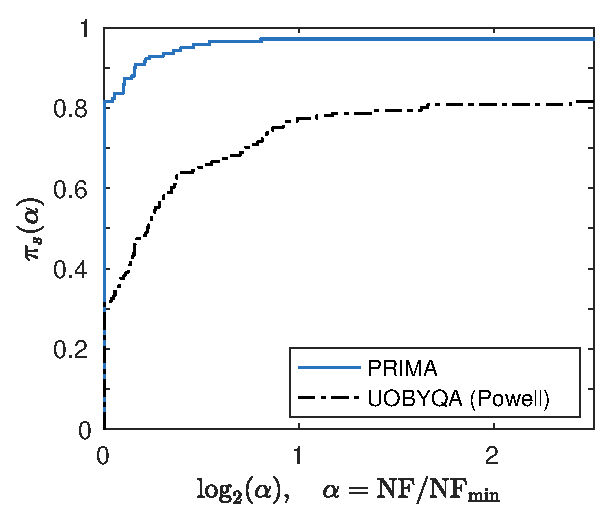
\includegraphics[width=0.5\textwidth]{prima_uobyqa.eps}
    \\[2ex]PRIMA v.s. UOBYQA \\[1ex](unconstrained problems, at most 100 variables)
    \end{center}
\end{frame}

%\begin{frame}
%    \frametitle{Performance of PRIMA compared with Powell's solvers}
%    \vspace{3ex}
%    \begin{center}
%    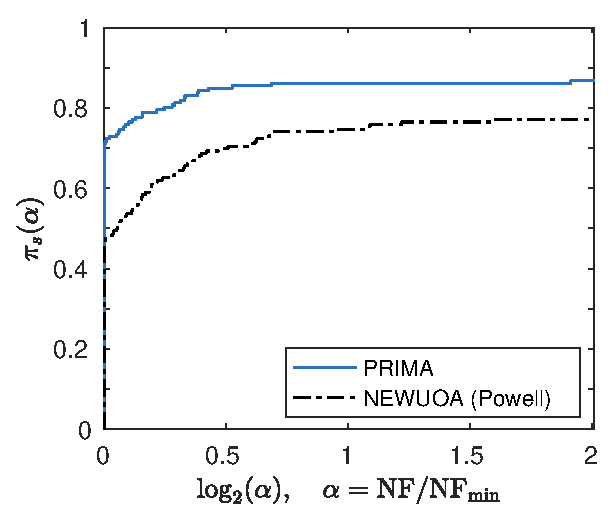
\includegraphics[width=0.5\textwidth]{prima_newuoa.eps}
%    \\[2ex]PRIMA v.s. NEWUOA \\[1ex](unconstrained problems, at most 200 variables)
%    \end{center}
%\end{frame}

\begin{frame}
    \frametitle{Performance of PRIMA compared with Powell's solvers}
    \vspace{3ex}
    \begin{center}
    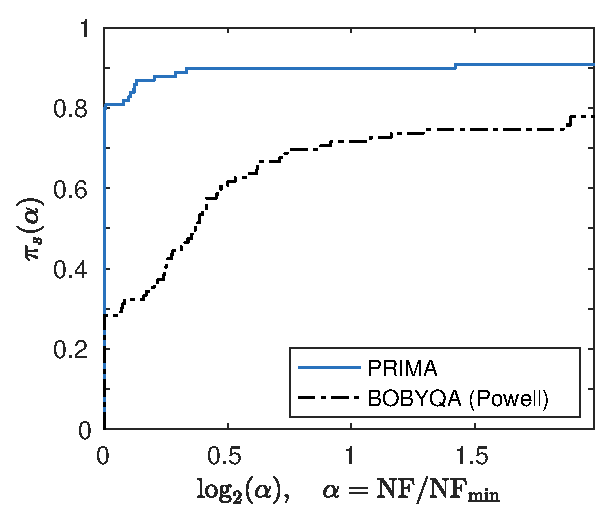
\includegraphics[width=0.5\textwidth]{prima_bobyqa.eps}
    \\[2ex]PRIMA v.s. BOBYQA \\[1ex](bound-constrained problems, at most 200 variables)
    \end{center}
\end{frame}

\begin{frame}
    \frametitle{Performance of PRIMA compared with Powell's solvers}
    \vspace{3ex}
    \begin{center}
    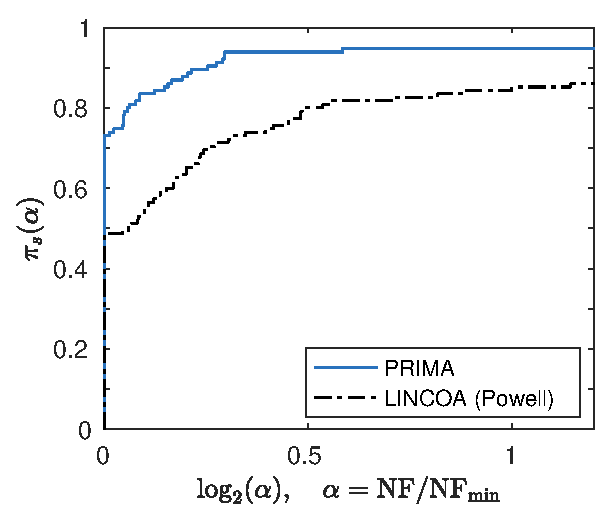
\includegraphics[width=0.5\textwidth]{prima_lincoa.eps}
    \\[2ex]PRIMA v.s. LINCOA \\[1ex](linearly constrained problems, at most 200 variables, 20,000 constraints)
    \end{center}
\end{frame}

\begin{frame}
    \frametitle{Performance of PRIMA compared with Powell's solvers}
    \vspace{3ex}
    \begin{center}
    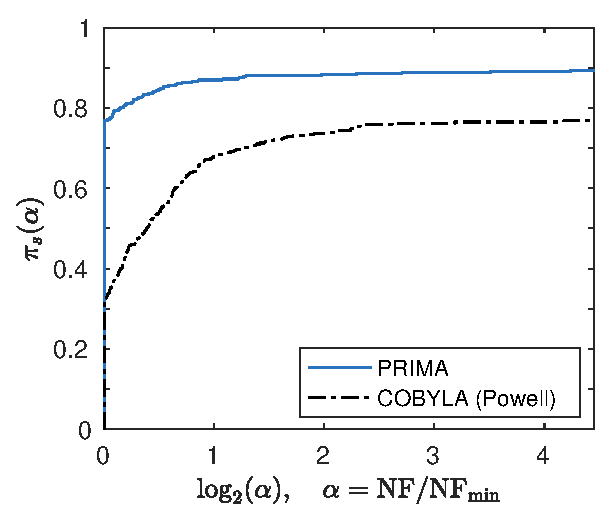
\includegraphics[width=0.5\textwidth]{prima_cobyla.eps}
    \\[2ex]PRIMA v.s. COBYLA \\[1ex]\mbox{\!\!(nonlinearly constrained problems, at most 100 variables,
    10,000 constraints)}
    \end{center}
\end{frame}


\begin{frame}
    \frametitle{Sorry, I lied ...}

    \vspace{10ex}
    Topics of this talk:
    \vspace{2ex}
    \begin{enumerate}
        \item \st{A new DFO solver named PRIMA}
            \\[1ex] \mbox{PRIMA is not a new solver but a \red{re}-implementation of Powell's solvers.}%
            \vspace{2ex}
        \item \st{The mathematics behind it}
            \\[1ex]
            There is no mathematics in this talk.
    \end{enumerate}

    \vspace{2ex}
\end{frame}

\begin{frame}
    \thispagestyle{empty}
    \vspace*{-10pt}
    \makebox[\linewidth]{
\includegraphics[width=\paperwidth]{titlepage.pdf}}
\end{frame}

\setcounter{framenumber}{0}

\begin{frame}
    \frametitle{Trust-region DFO methods based on interpolation models
    }
    \begin{figure}[htbp]
    \centering
    \only<1>{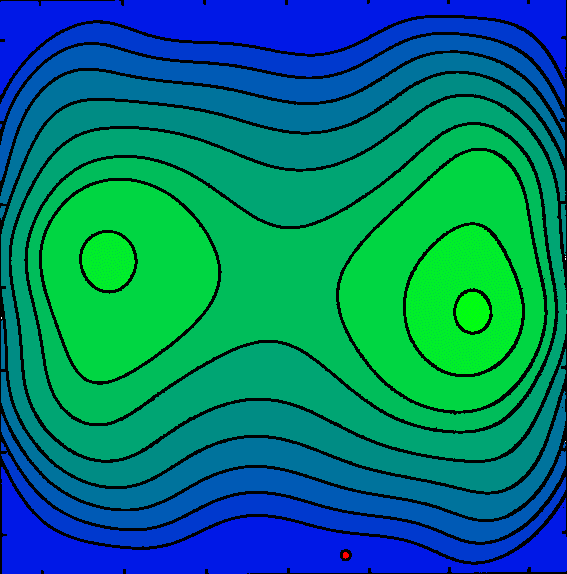
\includegraphics[width=0.2\textwidth]{tr00.png}}
    \only<2>{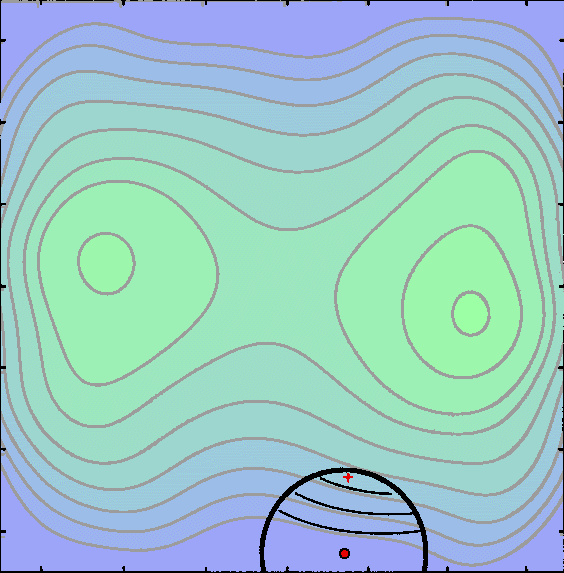
\includegraphics[width=0.2\textwidth]{tr01.png}}
    \only<3>{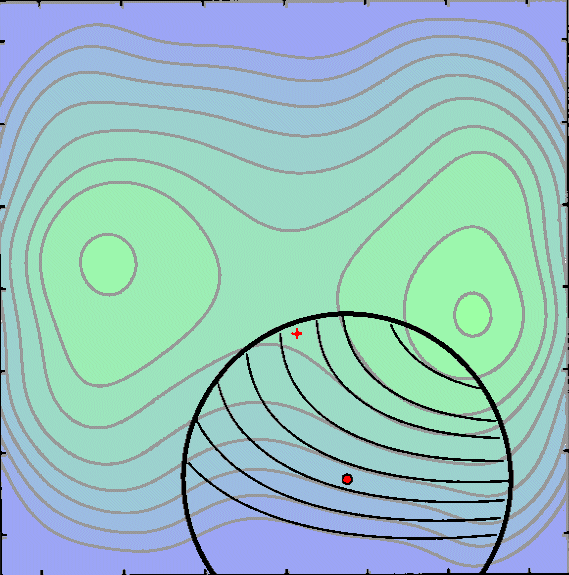
\includegraphics[width=0.2\textwidth]{tr02.png}}
    \only<4>{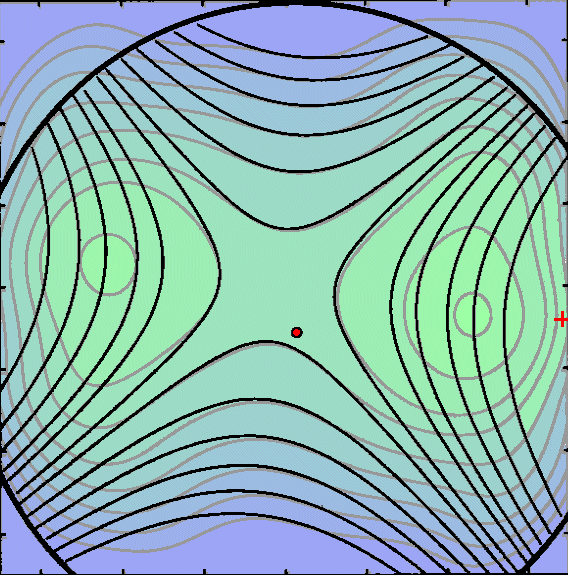
\includegraphics[width=0.2\textwidth]{tr03.png}}
    \only<5>{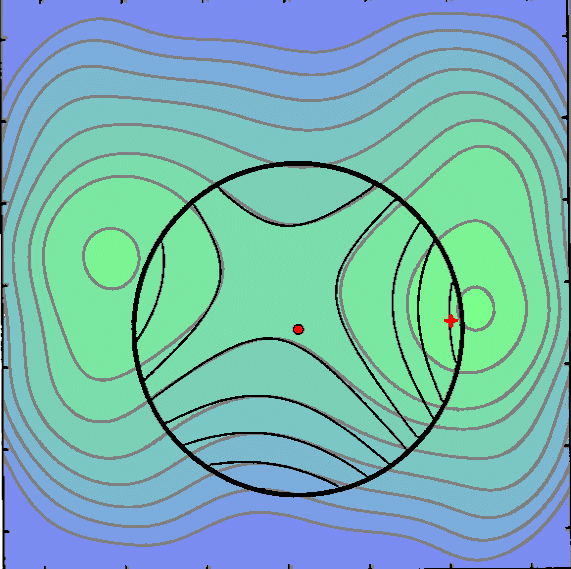
\includegraphics[width=0.2\textwidth]{tr04.png}}
    \only<6>{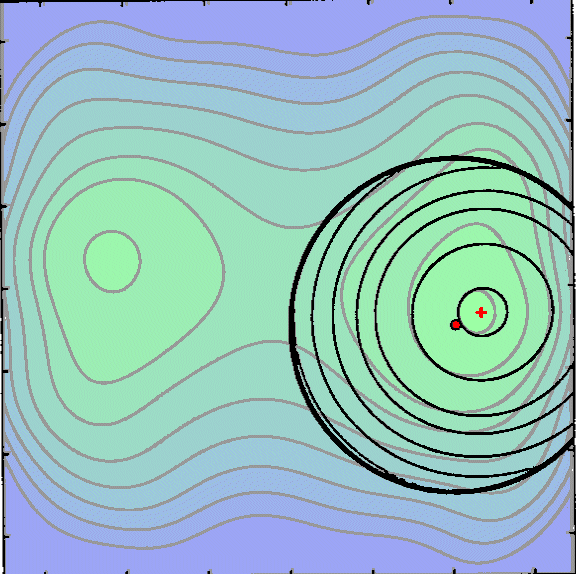
\includegraphics[width=0.2\textwidth]{tr05.png}}
\end{figure}
      %Objective function: $f(x,y) \;=\; -10x^2+10y^2+4\sin(xy) - 2x+x^4$
    %\vspace{-0.2ex}
    \hspace{2.25cm}
    \begin{beamerboxesrounded}[width=7cm,shadow=true]{}
    \begin{equation*}
        x_{k+1} \;\red{\approx}\; x_k + \rargmin_{\blue{\|d\|\le \Delta_k}}
      \blue{M_k(x_k+d)}
    \end{equation*}
    \end{beamerboxesrounded}
    \blfootnote{Images by Dr. F. V. Berghen from \url{http://www.applied-mathematics.net}.}
    \vspace{0.2ex}
\begin{itemize}
  \item $M_k$ is the trust-region model  (surrogate)
    \begin{itemize}
        \item \blue{$M_k(x)\approx f(x)$ around~$x_k$}
%      \item When derivatives are available: Taylor expansion or its variants %(Newton, quasi-Newton, ...)
      \item  $M_k$ interpolates $f$ on a set~\blue{$\mathcal{X}_k$ consisting of previous iterates}
    \end{itemize}
\vspace{0.6ex}
  \item \blue{$\|d\|\le\Delta_k$} is the \blue{trust-region} constraint
      \begin{itemize}
          \item If ``things work well'', increase~$\Delta_k$
          \item Otherwise, decrease~$\Delta_k$
          \end{itemize}
\end{itemize}

\end{frame}


\begin{frame}
    \frametitle{Maintenance of the interpolation set}
    \vspace{2ex}
    The interpolation set $\mathcal{X}_k$ must be updated with care.
    \vspace{1ex}
    \begin{itemize}
        \item $\mathcal{X}_k$ must \blue{reuse previous iterates} as much as possible.
    \vspace{1ex}
\item The \blue{geometry} of \mbox{$\mathcal{X}_k$ must ensure the well-conditioning of~the~problem}
            \[
                M_k(x) = f(x), \quad x \in \mathcal{X}_k.
            \]
    %\vspace{1ex}
\item Normally, $\mathcal{X}_{k+1} = \left(\mathcal{X}_{k}\cup\{x_{k+1}\}\right) \setminus\{\text{a ``bad'' point}\}$.
    \vspace{1ex}
\item Take \blue{geometry-improving steps} if the geometry of $\mathcal{X}_k$ deteriorates.
    \end{itemize}
\end{frame}

\begin{frame}
  \frametitle{Powell's trust-region DFO algorithms and software}

      \vspace{1ex}
      \begin{itemize}
          \item  COBY\red{L}A: solving general nonlinearly constrained problems using \red{linear} models; code released in 1992; paper published in 1994
      \vspace{1ex}

    \item  UOBYQA: solving unconstrained problems using quadratic models; code released in 2000; paper published in 2002
      \vspace{1ex}

    \item  NEWUOA: solving unconstrained problems using quadratic models; code released in 2004; paper published in 2006
      \vspace{1ex}

    \item  BOBYQA:
       solving bound-constrained problems using
       quadratic models; code released and paper written in 2009

      \vspace{1ex}
     \item  LINCOA:
       solving linearly constrained problems using
       quadratic models; code released in 2013 but no paper written

       \vspace{1ex}
       \pause
       \item What about \red{COBYQA}? %--- That's \blue{Tom Ragonneau}'s talk.
  \end{itemize}
\end{frame}

%\begin{frame}
%    \frametitle{What do these algorithms look like?}
%    \vspace{-2ex}
%\begin{center}
%    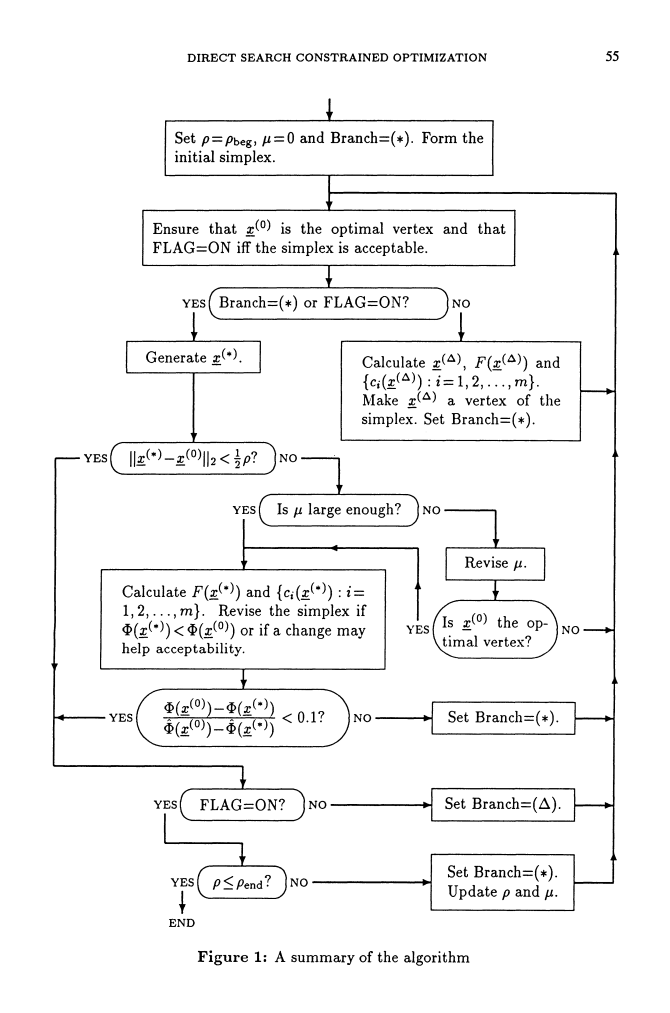
\includegraphics[width = 0.42\textwidth]{cobyla_alg.png}
%    \\COBYLA
%\end{center}
%\end{frame}


\begin{frame}
    \frametitle{What do these algorithms look like?}
    \vspace{-2ex}
\begin{center}
    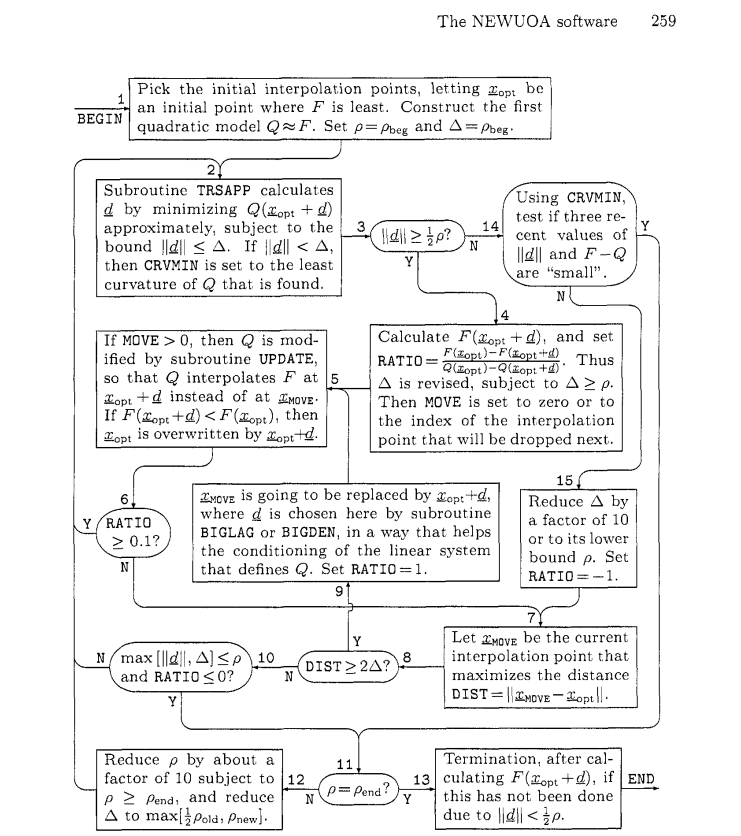
\includegraphics[width = 0.55\textwidth]{newuoa_alg.png}
    \\[1ex]NEWUOA
\end{center}
\end{frame}


\begin{frame}
    \frametitle{Implementation of these methods is HARD}
    \vspace{3ex}
    \begin{mybox}
    \textnormal{The development of NEWUOA has taken nearly \red{three} years. The work
    was very \red{frustrating} ...
}
\end{mybox}
    \begin{flushright}
        --- {M. J. D. Powell}
    \vspace{0.3ex}
    \\\small{The NEWUOA software for unconstrained optimization without derivatives, 2006}
    \end{flushright}

    \nb
    \begin{itemize}
        \item NEWUOA was Powell's \blue{third} trust-region DFO solver, COBYLA and UOBYQA being the first two.
    \vspace{0.3ex}
\item Mathematically speaking, NEWUOA and UOBYQA are \blue{essentially the same except for the
    ways they construct the model}.
    \vspace{0.3ex}
\item Given the experience with UOBYQA (and COBYLA), Powell still spent \red{three frustrating
        years} on the development of NEWUOA.
    \end{itemize}
\end{frame}

\begin{frame}
    \frametitle{The central difficulty}
    \vspace{6ex}
    \begin{center}
    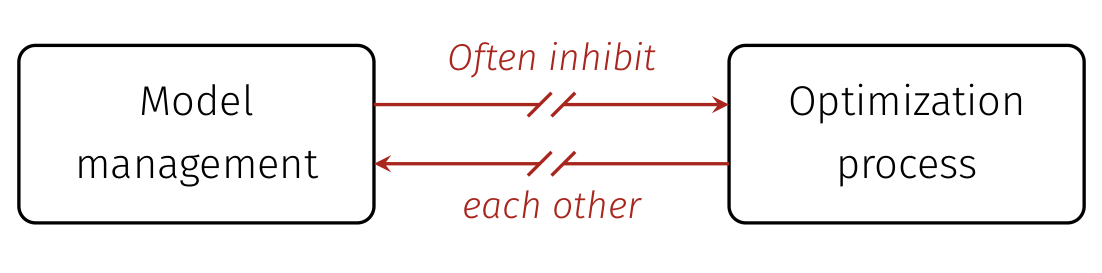
\includegraphics[width=0.8\textwidth]{difficulty.png}
    \end{center}
\end{frame}


\begin{frame}
    \frametitle{Powell's implementation}

            \vspace{2ex}
    \begin{itemize}
        \item Powell implemented these five methods into publicly available~solvers.%
    \vspace{1ex}
\item The solvers are \blue{widely used by scientists and engineers}.
    \vspace{1ex}
\item They are often used as \blue{benchmarks} when designing new algorithms.
    \vspace{1ex}
        \item However, the implementation was in \red{Fortran 77}, with plenty of \red{GOTO}s:
            in total,  \red{7939} lines of code with \red{249} GOTOs!
    \end{itemize}

    \begin{center}
    \red{A modernized implementation is greatly needed.}
    \end{center}
\end{frame}

\begin{frame}
    \frametitle{Why should \textbf{\textrm{I}} work on a modernized implementation}

            \vspace{2ex}
    \begin{itemize}
        \item Professor Powell, April 2015: ``It would be a relief to me if you would kindly continue
            to look after my optimisation software (NEWUOA, BOBYQA and LINCOA). Also I would like
            you to add COBYLA and TOLMIN if you do not have them already.''
            \vspace{1ex}
        \item Stefan Wild, ICCOPT 2016, Tokyo: People do not want interfaces. They want
            implementations that they can understand and play with.
            \vspace{1ex}
        \item Jeff Larson, ISMP 2018, Bordeaux: Numerical linear algebra people have standard
            implementations for standard algorithms, e.g., LAPACK, whereas we all work on our own
            implementation of interpolation, model improvement, ...
    \end{itemize}
\end{frame}

\begin{frame}
    \frametitle{Isn't it a perfect project for an engineer or a student?}

    \begin{itemize}
            \vspace{2ex}
        \item Given that \blue{Powell spent three frustrating years} on the development of \red{his own
            algorithm} NEWUOA despite his abundant experience, where could I find this
            \blue{genius engineer} who can learn all the \blue{five} algorithms \red{from scratch} and implement them in
            a reasonable amount of time?
            \vspace{0.5ex}
        \item Assume that I am lucky to find the abovementioned \blue{genius engineer} and he/she happens
            to be my Ph.D. student. How should I persuade him/her to be \blue{fully devoted to
            a project for three years}~(as I did) \red{without producing a single publication}? Am I even allowed to do so?
        %    \vspace{0.5ex}
        %\item What about hiring multiple engineers or students to work on this project in parallel
        %    (suppose that they can be \blue{``hired'' for free})? You are assuming that the project is
        %    a simple \blue{engineering project} that can be easily divided into \blue{small tasks}.
        %    No. It is a \red{research project} that I do not know how to do it until I have done it.
        %    \vspace{0.5ex}
        %\item After all, \blue{if the project was easy, someone else would have done it years ago, and I would
        %    not even have the opportunity to work on it.}
    \end{itemize}
\end{frame}


%\begin{frame}
%    \frametitle{PRIMA is not PDFO}

%    \vspace{1ex}

%    \begin{itemize}
%        \item PRIMA is not PDFO (T. M. Ragonneau and Z.), which provides interfaces to
%            \blue{Powell's original Fortran 77 code}.
%            \vspace{1ex}
%        \item PRIMA would have been a mission impossible without PDFO.
%    \end{itemize}

%    \vspace{1ex}

%    We received requests for modifying Powell's code after releasing PDFO. \\My typical response is
%    as follows.
%    \begin{mybox}
%        \textnormal{\small Before finishing the re-implementation [PRIMA], we refrain from making any
%            changes to Powell's code.
%           Due to the unique coding style, \red{Powell's code has extremely high complexity} --- I would
%            say that \red{nobody can see the true complexity before trying to disentangle the GOTOs}, ...
%    Consequently, changing one place will inevitably affect many other places,
%    ... sometimes in a way that is hard to imagine ...
%    \blue{Making changes to such code is like
%    introducing new components in a machine that has already excessively many interconnected wires,
%buttons, knobs, and switches.} This may do some good, but I guess it is better to postpone the
%    changes until the machine is modularized and the structure becomes clearer.
%}
%\end{mybox}

%\end{frame}


\begin{frame}
    \frametitle{PRIMA}

    \begin{center}
    \qrcode[height=0.15\textwidth]{http://www.libprima.net}
    \\[1.6ex]\href{http://www.libprima.net}{\blue{\texttt{libprima.net}}}
    \end{center}
    %\begin{columns}[T]
    \vspace{1ex}
    PRIMA is an acronym for
    \begin{center}
        ``Reference Implementation for Powell's Methods \\with Modernization and Amelioration'',
    \end{center}
    \blue{``P'' for Powell}.
\end{frame}

\begin{frame}
    \frametitle{An inspiration}

    \begin{center}
        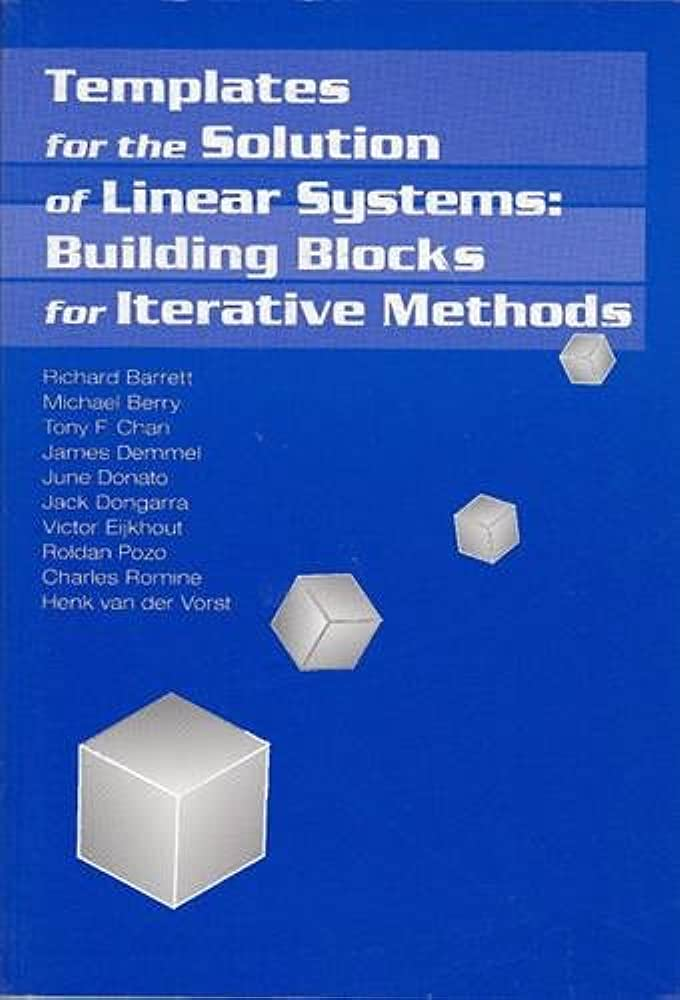
\includegraphics[width=0.4\textwidth]{linalg.jpg}
    \end{center}

\end{frame}



\begin{frame}
    \frametitle{An overview of PRIMA}
\begin{itemize}
    \item The solvers are implemented in a structured and modularized way so that they are
        \blue{understandable}, \blue{maintainable},
        \blue{extendable},  \blue{fault-tolerant}, and~\mbox{\blue{future-proof}}.
    \vspace{1ex}
\item The code has \blue{no GOTO} and \blue{uses matrix-vector procedures instead of loops} whenever possible.
    \vspace{1ex}
\item The implementation is \blue{mathematically equivalent} to Powell's \red{except for the bug
    fixes and improvements we introduce intentionally}.
    \vspace{1ex}
\item The implementation of PRIMA in \blue{modern} Fortran (F2008 or above) has been finished.
    \vspace{1ex}
\item Versions in MATLAB, Python, Julia, R, ... will be implemented using the \blue{modern} Fortran as a reference.
    \vspace{1ex}
\item A MATLAB interface is provided to use the \blue{modern} Fortran version.
    \vspace{1ex}
\item The \red{inclusion of PRIMA into SciPy} is under discussion, and the major SciPy maintainers are
    positive about it.
\end{itemize}
\end{frame}


\begin{frame}
    \frametitle{Why do I start with modern Fortran?}

    \begin{center}
    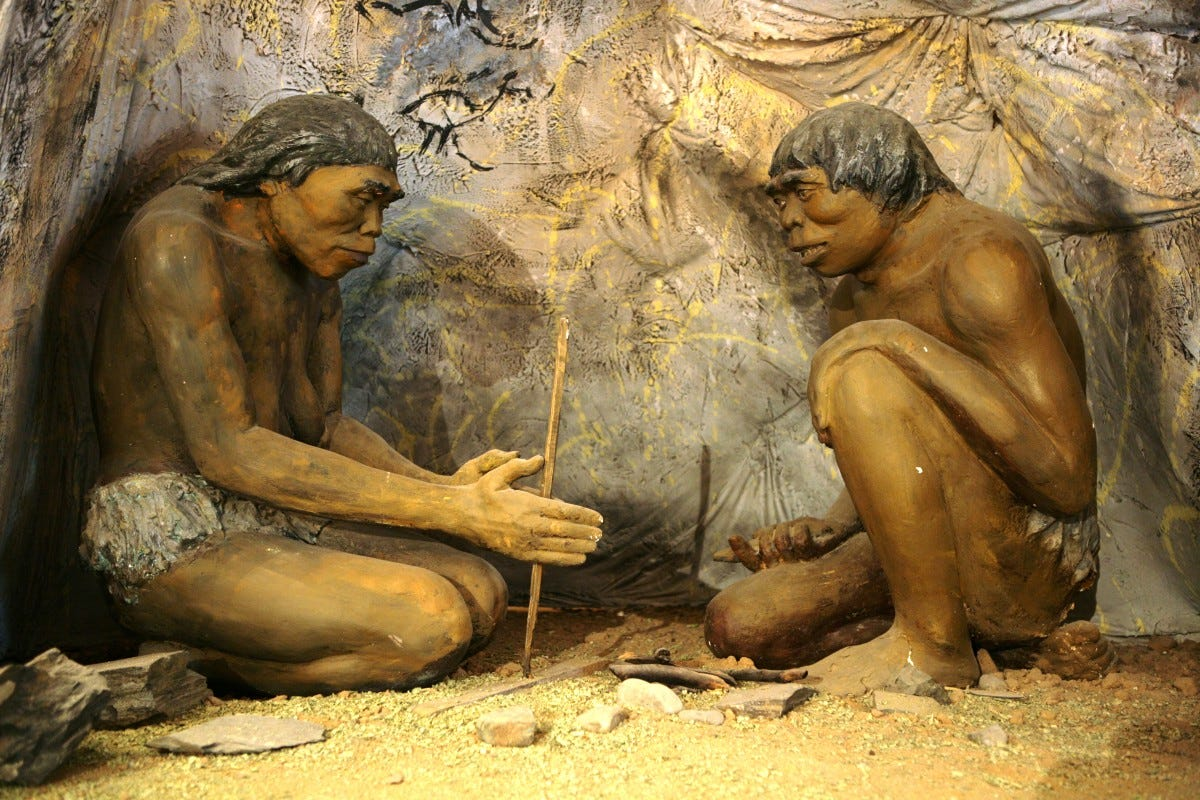
\includegraphics[width=0.4\textwidth]{caveman.jpg}
    \\[1ex]{Fortran? Are you a caveman?}
    \end{center}

    \begin{itemize}
        \item The syntax and style of \blue{modern} Fortran are very similar~to~MATLAB.
            \vspace{0.5ex}
        \item I \red{start} with modern Fortran, so that I can \blue{systematically verify} the
            \red{bit-to-bit faithfulness} of PRIMA,  as the original code is Fortran.%
            \vspace{0.5ex}
        \item With other languages,~the verification is hard,~if not impossible.%~\!(\red{Why?})}%
    \end{itemize}

 \begin{mybox}
    \begin{center}
        \textnormal{
            Ultimate goal of PRIMA: \\
            Make Powell's methods \blue{available to everyone in her/his favorite languages}.
        }
    \end{center}
\end{mybox}


\end{frame}


\begin{frame}
    \frametitle{Powell's description of NEWUOA (recapped)}
    \vspace{-2ex}
\begin{center}
    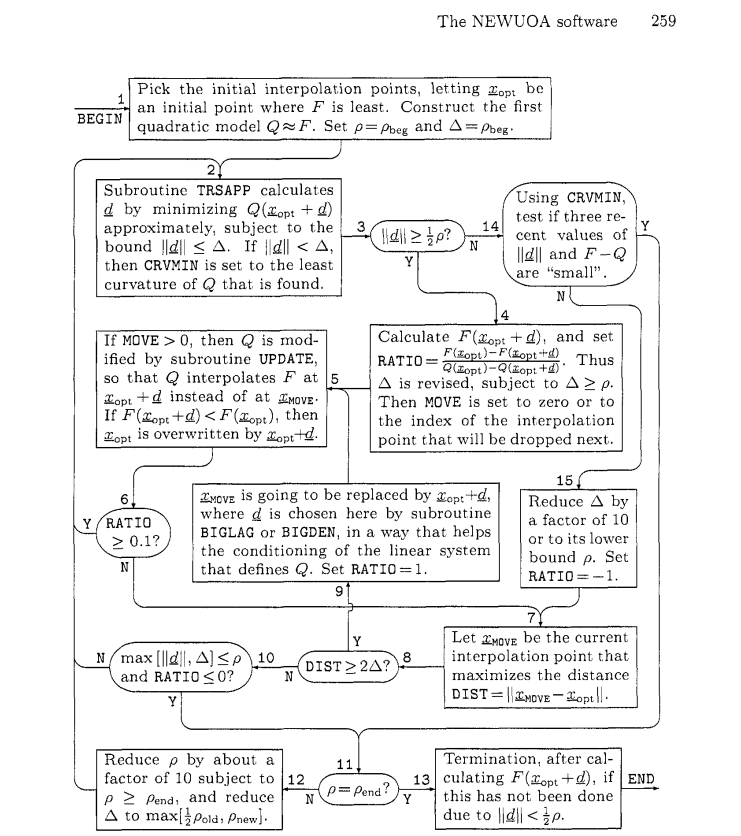
\includegraphics[width = 0.55\textwidth]{newuoa_alg.png}
    \\[1ex]NEWUOA
\end{center}
\end{frame}


\begin{frame}
    \frametitle{The original implementation of NEWUOA: a snippet}
    \vspace{-1ex}
    \begin{center}
        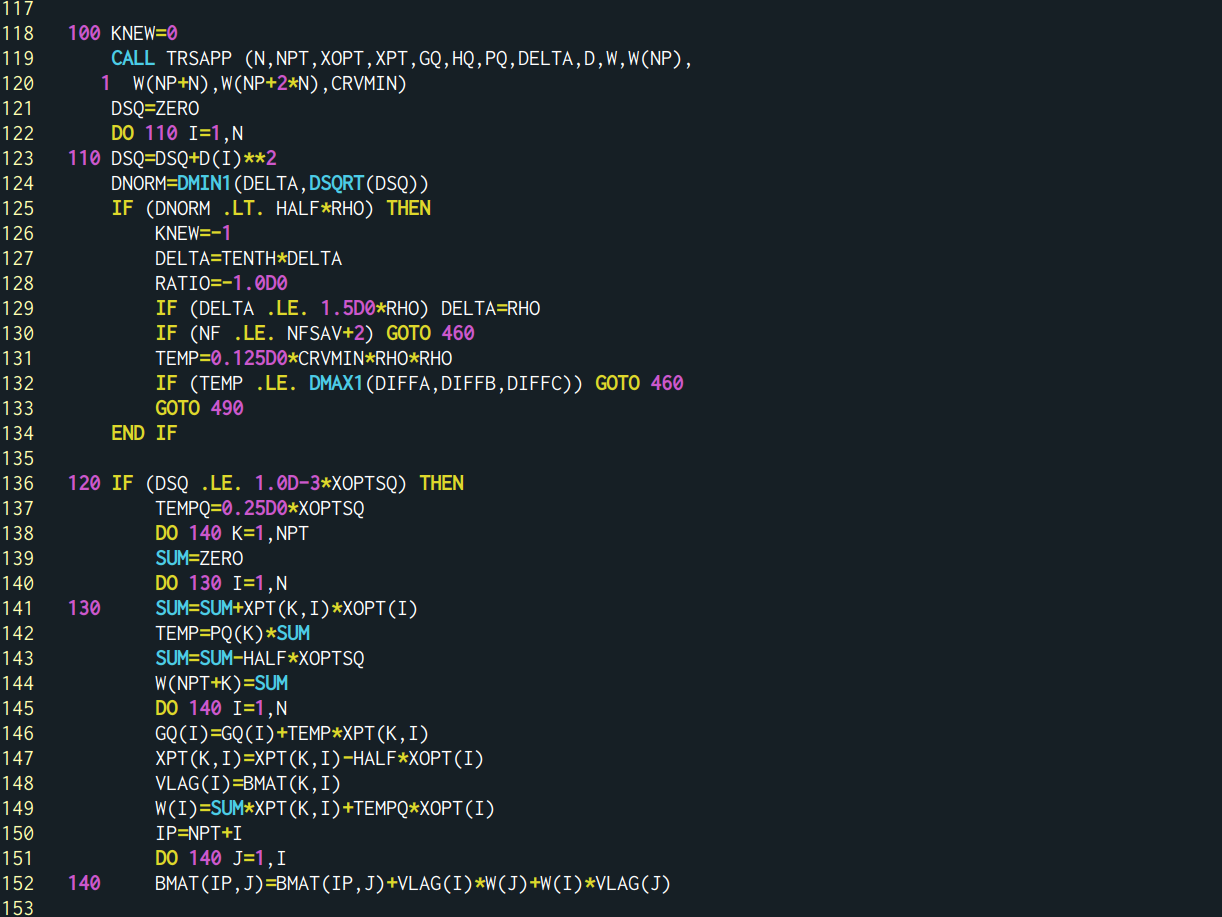
\includegraphics[width=0.9\textwidth]{newuoa_orig.png}
    \end{center}
\end{frame}

\begin{frame}[fragile]
    \frametitle{\textbf{Faithful} pseudocode of NEWUOA in PRIMA}
    \vspace{-1.1ex}
\textnormal{\small
    \mbox{Pick $\XX\!\subset\!\RR^n$ and $\rho > 0$. Let $M$ interpolate~$f$ on~$\XX$.~\blue{$x_\opt
    := \argmin_{x\in\XX}f(x)$}. $\Delta := \rho$.}
\vspace{-3ex}
\begin{algorithmic}[1]
\WHILE{not converged}
\STATE Calculate a \blue{trust-region trial point} $x_\tr \approx \argmin\{M(x)\mathrel{:}  \|x-x_\opt\|\le \Delta\}$
\IF{$M(x_\opt)-M(x_\tr)$ is too small or $\|x_\tr-x_\opt\|$ is too short}
\STATE Reduce $\Delta$ \red{subject to $\Delta \ge \rho$}
\ELSE
\STATE Evaluate the \blue{reduction ratio} and \blue{update $\Delta$ accordingly} \red{subject to $\Delta \ge \rho$}
\IF{it is proper to replace a point~$x_{\drop}\in\XX$ with $x_\tr$}
\STATE Set \blue{$\XX = \big(\XX \cup \{x_\tr\}\big) \setminus\{x_\drop\}$}, and then \blue{update $M$ and~$x_\opt$}% to interpolate~$f$ on~$\XX$
\ENDIF
\ENDIF
\STATE $\blue{\texttt{improve\_geo}} := x_\tr \text{ is bad}~\&~\text{the geometry of } \XX \text{ is inadequate}$
\STATE $\blue{\texttt{reduce\_rho}}~\,:= x_\tr  \text{ is bad}~\&~\text{the geometry of } \XX \text{ is adequate}~\&~\Delta \text{ is small}$
\IF{\texttt{improve\_geo}}
\STATE Decide a point~$x_{\drop}\in\XX$ to drop and a \blue{geometry-improving point}~$x_\geo$
\STATE Set \blue{$\XX = \big(\XX \setminus\{x_\drop\}\big)\cup\{x_\geo\}$}, and then \blue{update $M$ and~$x_\opt$}% to interpolate~$f$ on~$\XX$
\ENDIF
\STATE\textbf{if} {\texttt{reduce\_rho}} \textbf{then} reduce~$\rho$ and reduce $\Delta$
\red{subject to $\Delta \ge \rho$}
\ENDWHILE
\end{algorithmic}
\vspace{-0.6ex}
\nb: The \blue{updates} keep $M$ interpolating $f$ on~$\XX$ and $x_\opt = \argmin_{x\in\XX}f(x)$.
}
\end{frame}


\begin{frame}
    \frametitle{PRIMA NEWUOA: trust-region phase (ln.~2--10)}
    \vspace{-2.2ex}
    \begin{center}
        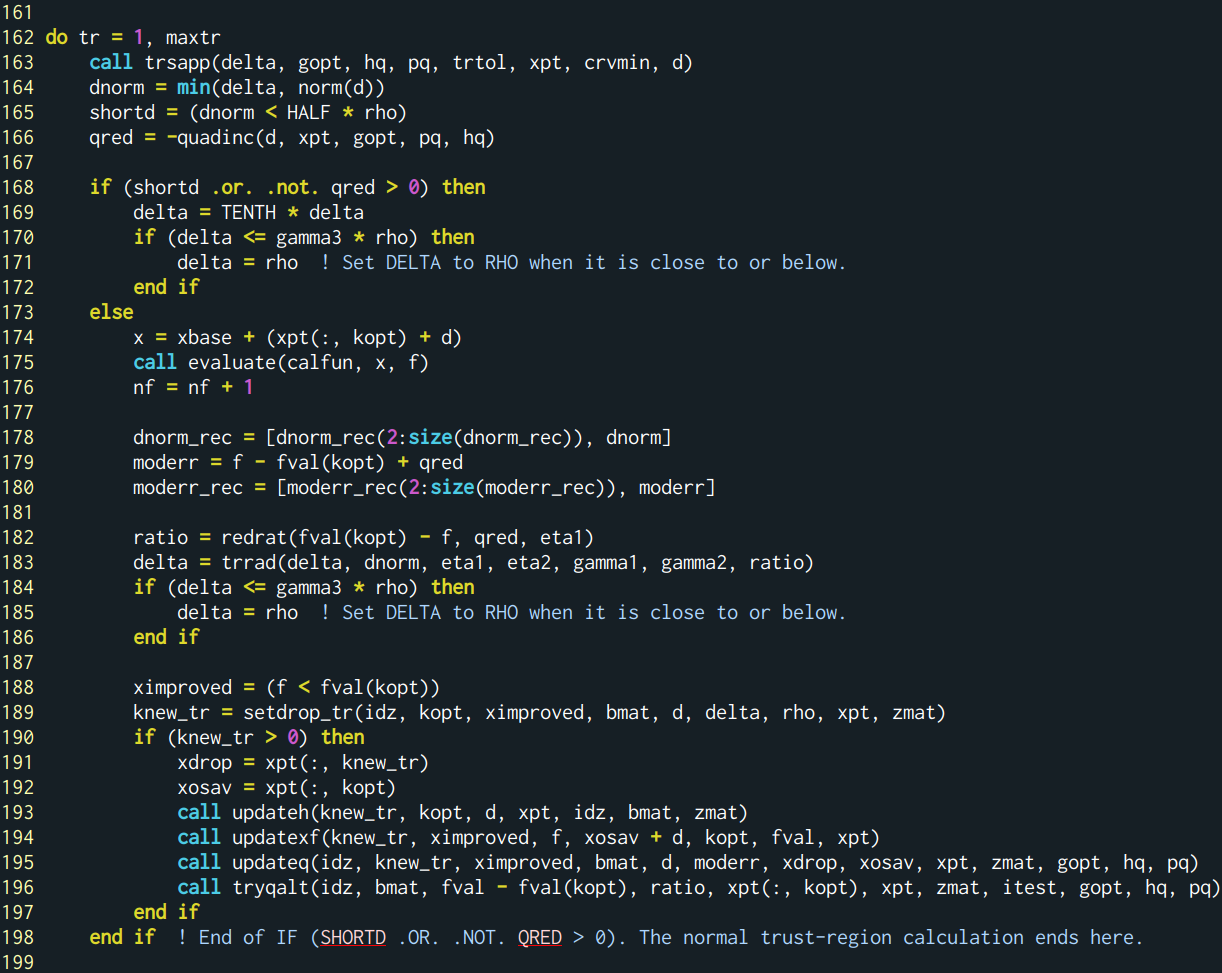
\includegraphics[width=0.9\textwidth]{newuoa_tr.png}
    \end{center}
\end{frame}

\begin{frame}
    \frametitle{\mbox{PRIMA NEWUOA: \texttt{improve\_geo}, \texttt{reduce\_rho} (ln.~\!11,\! 12)}}
    \vspace{12ex}
    \begin{center}
        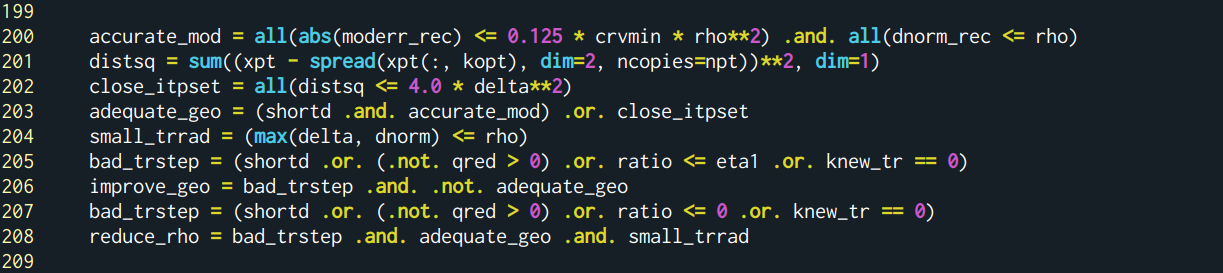
\includegraphics[width=0.9\textwidth]{newuoa_geo_rho.png}
    \end{center}
\end{frame}

\begin{frame}
    \frametitle{PRIMA NEWUOA: post-processing phase (ln.~13--17)}
    \vspace{-2ex}
    \begin{center}
        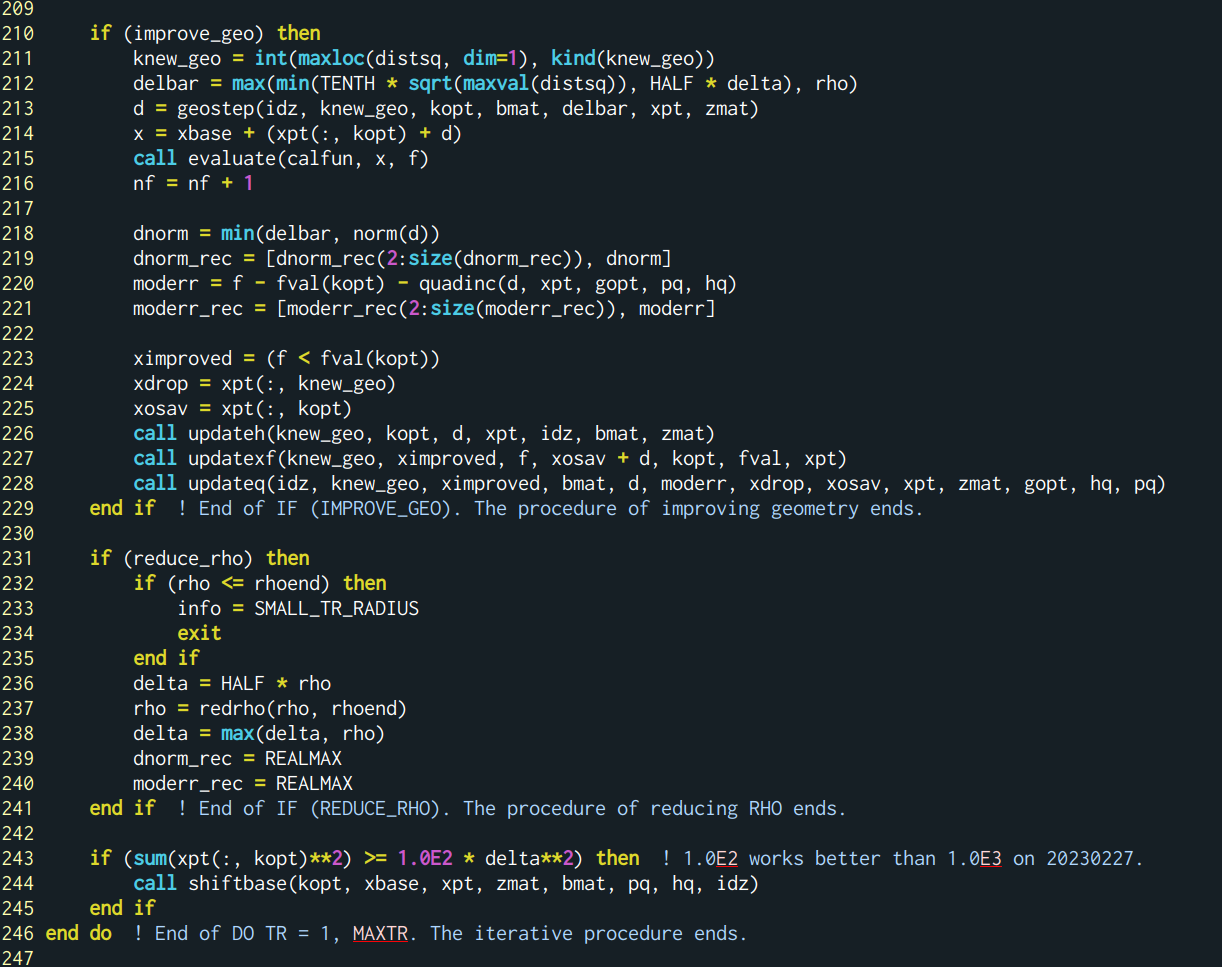
\includegraphics[width=0.9\textwidth]{newuoa_post.png}
    \end{center}
\end{frame}

\begin{frame}
    \frametitle{Issues in the Fortran 77 implementation: an example}
    \vspace{-1ex}
    \begin{center}
        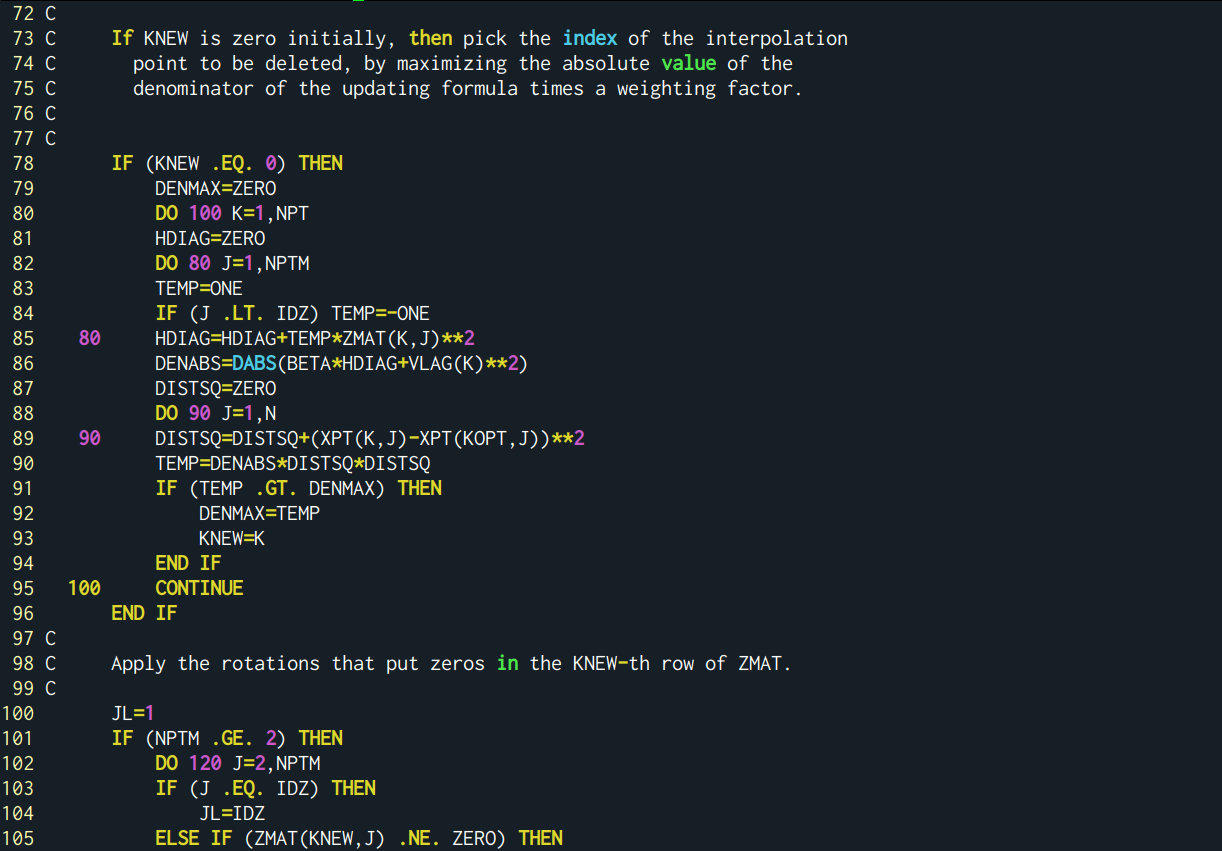
\includegraphics[width=0.9\textwidth]{lincoa_knew.png}
        \\[0.2ex]The above code may \red{crash}, as \texttt{KNEW} may be used uninitialized.
    \end{center}
\end{frame}

\begin{frame}
\frametitle{Issues in the Fortran 77 implementation}

    \vspace{1ex}
    \begin{itemize}
        \item\mbox{The Fortran 77 solvers may \red{crash with memory violations}~(segfaults).}
        \\Reason: Some indices are only initialized under conditions that can never be met because
        of~\blue{NaN} resulted from  \blue{floating point exceptions}.
        \vspace{0.5ex}
    \item The Fortran 77 solvers may \red{get stuck in infinite loops}.
        \\Reason: Some loops are only terminated under conditions that can never be met because
        of~\blue{NaN} resulted from  \blue{floating point exceptions}.
    \end{itemize}

    \vspace{1ex}
    \nb:
    \begin{itemize}
     \item The problems are due to floating point exceptions in the Fortran 77 code rather than flaws in the algorithms.
         \vspace{0.5ex}
     \item The problems affect all implementations or wrappers of these solvers based on the Fortran 77
         code, including \blue{SciPy} (COBYLA), \blue{NLopt}, ...
    \end{itemize}
\end{frame}

%\begin{frame}
%    \frametitle{Issues in the Fortran 77 implementation: suboptimal return}
%    Issue: The Fortran 77 version of COBYLA may not return the best point that is evaluated; sometimes, the
%            returned point can have a large constraint violation even though the starting point is feasible.
%      \\Reason: The way that Fortran-77 COBYLA chooses the returned point is not ideal. It
%            chooses the best point in the last interpolation set, even though better iterates may exist.
%\end{frame}

\begin{frame}
    \frametitle{How to ensure PRIMA does not have similar issues? }
    \textbf{Strategy 1.} Programming by contract
    \begin{center}
    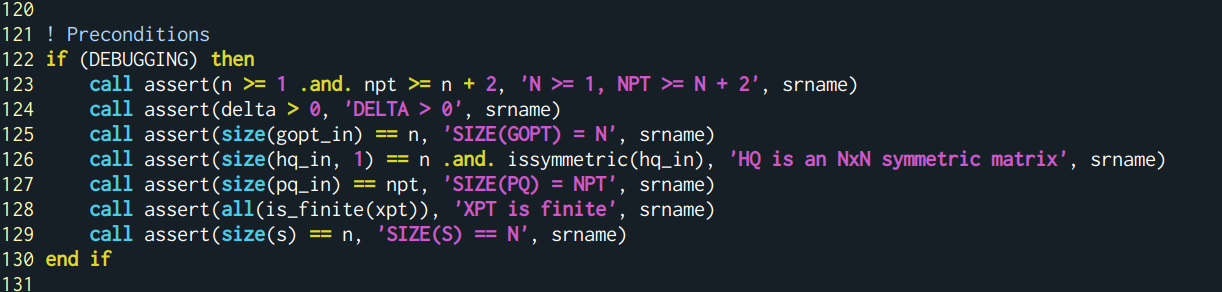
\includegraphics[width=0.9\textwidth]{newuoa_preconditions.png}
    \end{center}

    \begin{center}
    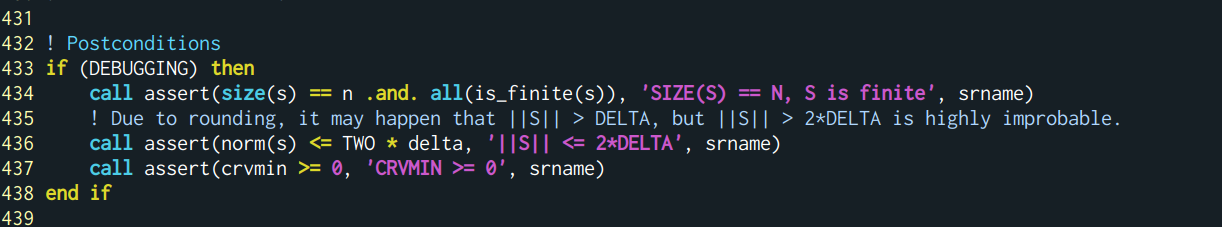
\includegraphics[width=0.9\textwidth]{newuoa_postconditions.png}
    \end{center}

    \begin{itemize}
        \item The preconditions and postconditions are \blue{checked} only in the \blue{debug mode}.
            In the code that users receive, they are disabled by default.%
            \vspace{0.5ex}
        \item
            In the debug mode,
            if some subroutine receives strange inputs or produces strange outputs, the program
            will \blue{raise an error} so that the developer (i.e., Zaikun Zhang) can \blue{check the issue and fix it}.
    \end{itemize}
\end{frame}

\begin{frame}
    \frametitle{How to ensure PRIMA does not have similar issues? }

    \textbf{Strategy 2.} TOUGH (Tolerance Of Untamed and Genuine Hazards) tests

    \begin{center}
        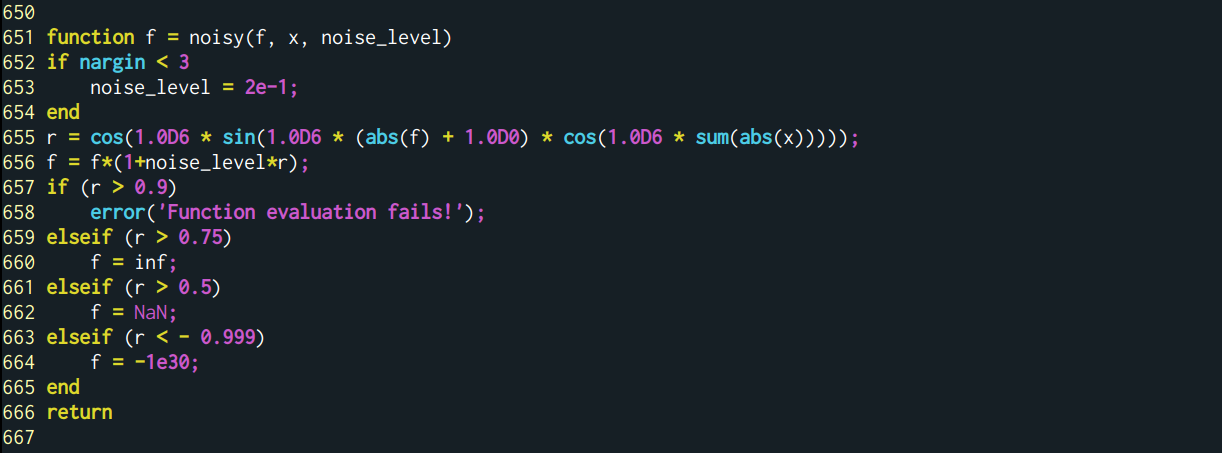
\includegraphics[width=0.9\textwidth]{tough.png}
    \end{center}

    \begin{itemize}
        \item In TOUGH tests, objective functions are corrupted as above and then fed to the solvers.
            \vspace{0.5ex}
        \item We make sure that PRIMA solvers work properly even if the objective functions are
            corrupted in this severe way. (\blue{What about your solvers?})
    \end{itemize}
\end{frame}


\begin{frame}
    \frametitle{How to ensure PRIMA does not have similar issues? }

    \vspace{2ex}
    \textbf{Strategy 3.} \blue{Automated and randomized} tests using \blue{GitHub Actions}
    \vspace{1ex}
    \begin{itemize}
        \item Every day, extensive TOUGH tests and other tests are conducted \blue{automatically}
            on \blue{randomized} variants of CUTEst problems.
    \vspace{1ex}
    \item The longer time passes, the more reliable PRIMA is, \blue{automatically}.
    \vspace{1ex}
        \item As of June 2023, $>$ 42,000 workflows have been successfully run.
    \vspace{1ex}
        \item Each workflow consists of $\sim$ 5 (sometimes more than 150) randomized tests,
            each test taking from tens of minutes to several hours.
    \vspace{1ex}
\item In other words, PRIMA has been verified by more than 200,000 hours (or \red{more than 20 years}) of randomized tests.
    \end{itemize}

    \vspace{1ex}
    \begin{center}
    \red{Code must be battle-tested before it becomes software.}
    \end{center}

\end{frame}


\begin{frame}
    \frametitle{The performance of PRIMA}
    \vspace{3ex}
    \begin{center}
    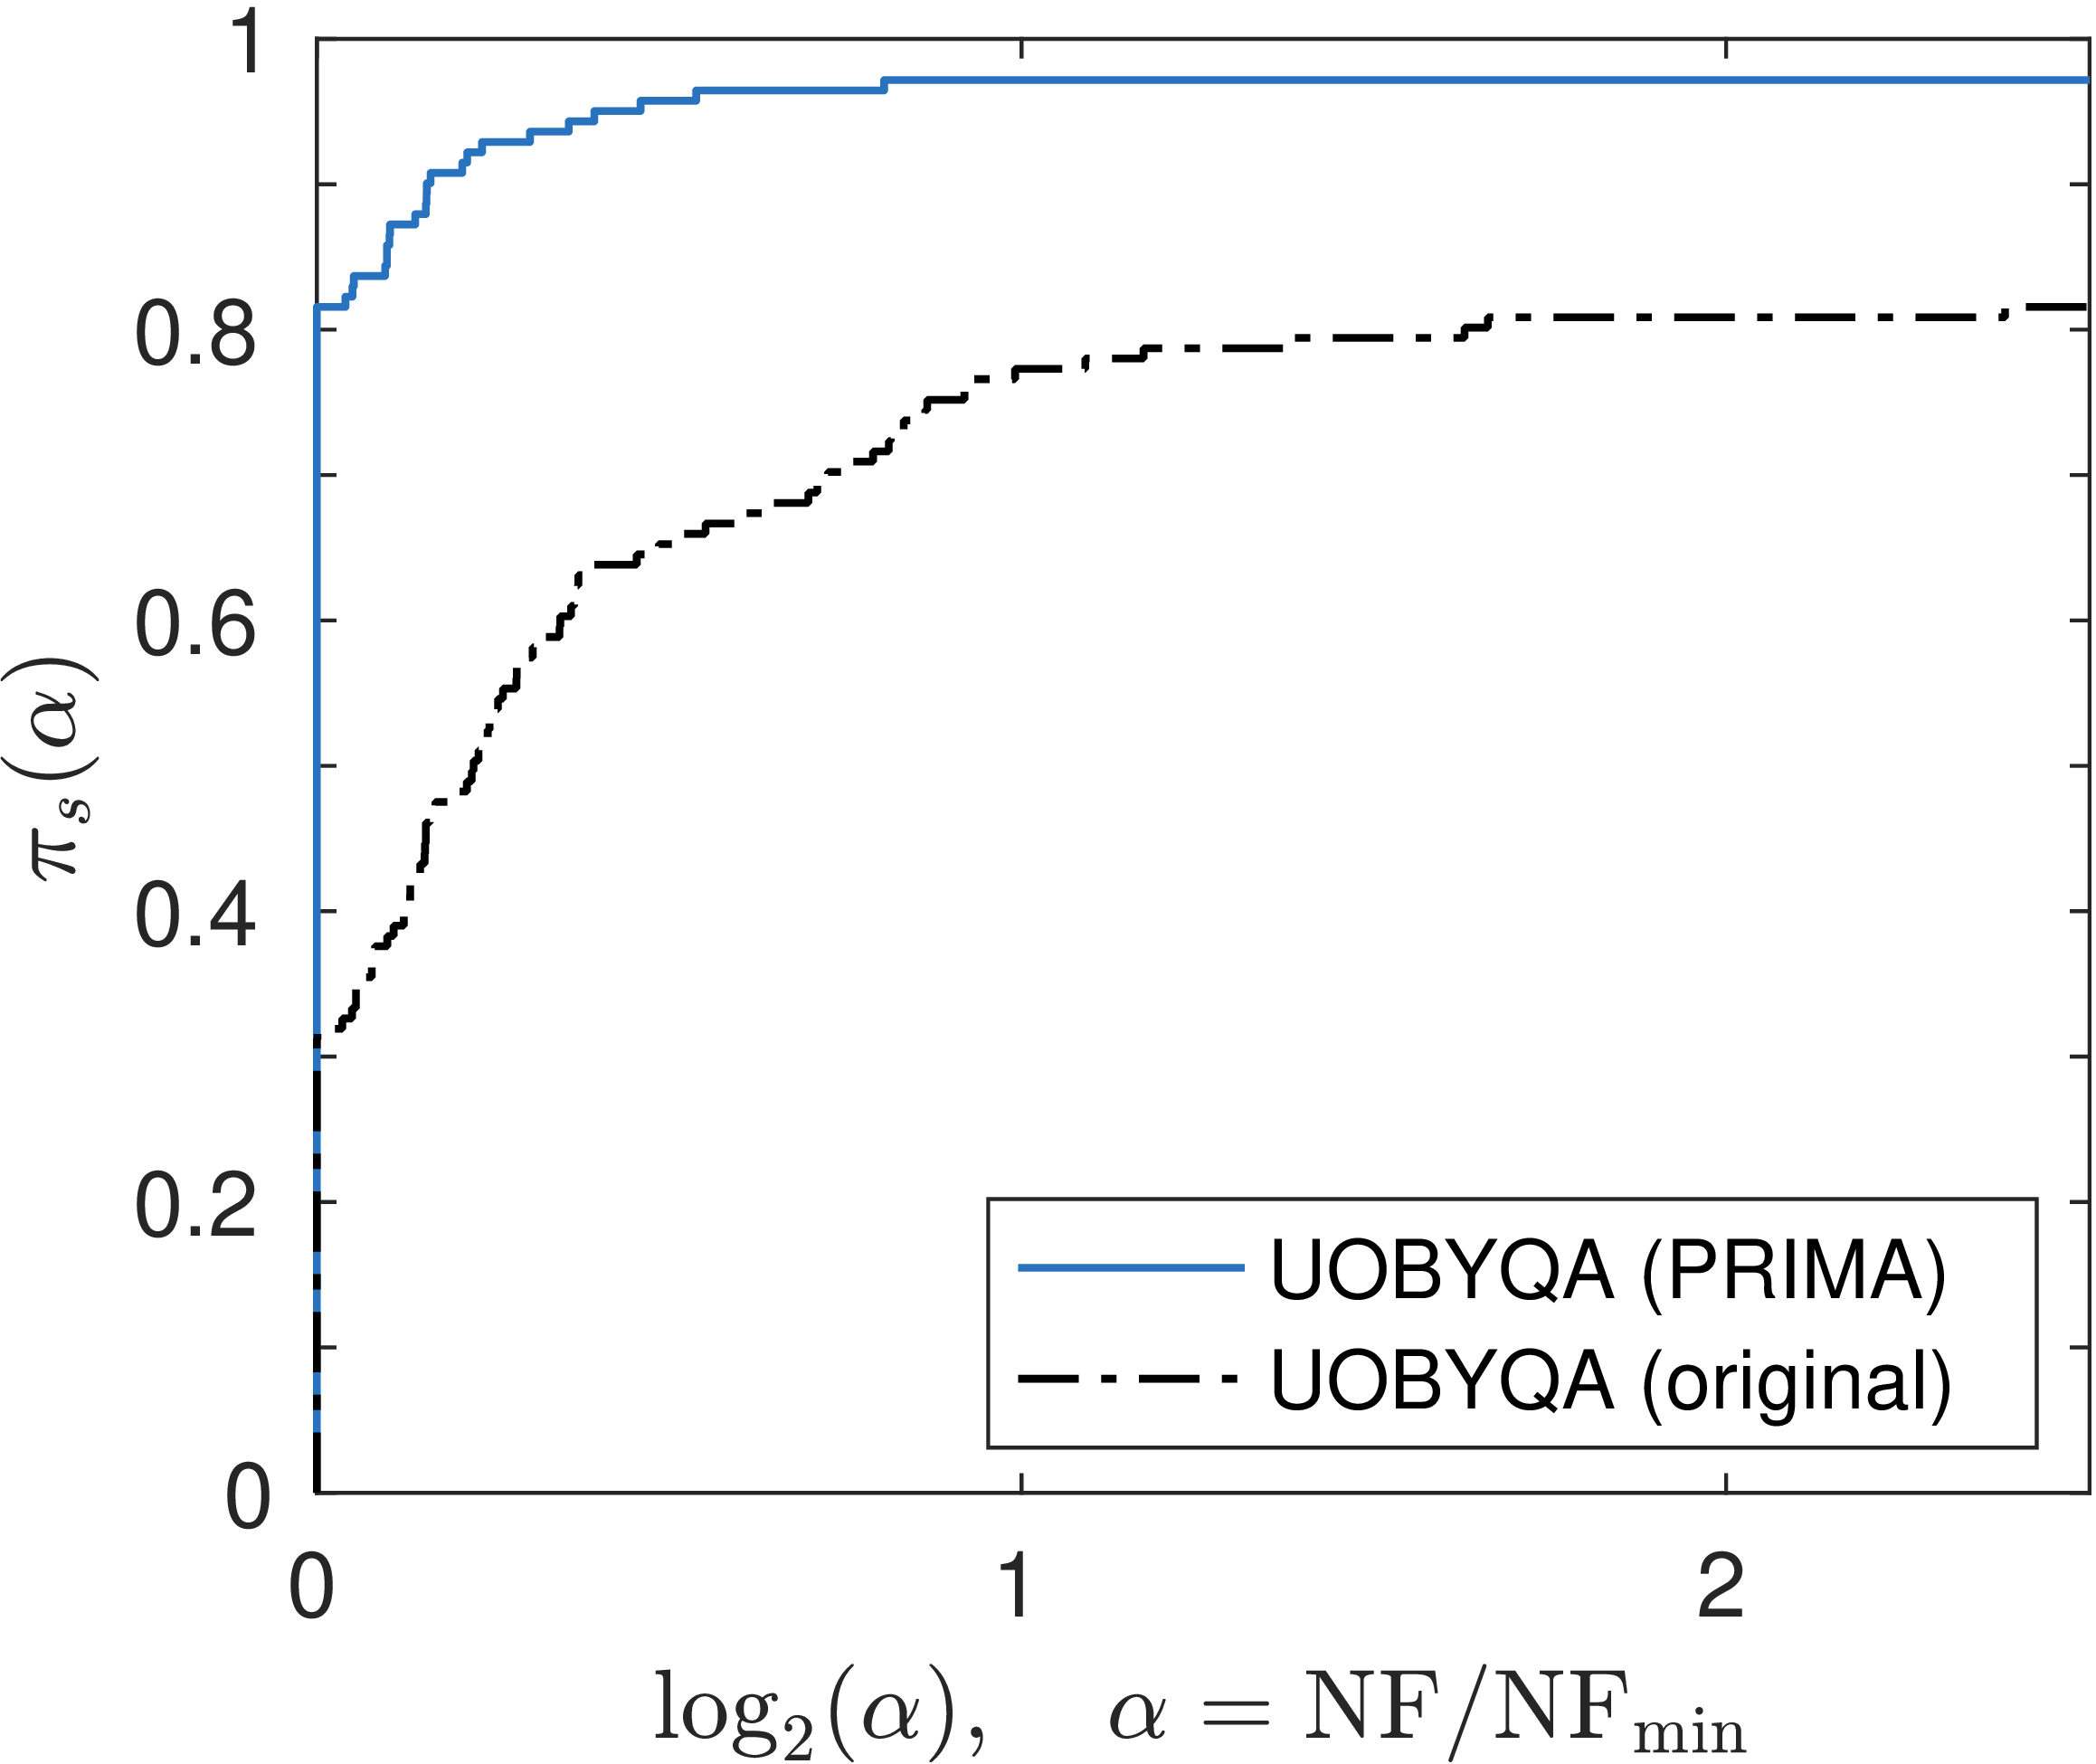
\includegraphics[width=0.5\textwidth]{prima_uobyqa.png}
    \\[2ex]UOBYQA \\[1ex](unconstrained problems, at most 100 variables)
    \end{center}
\end{frame}

\begin{frame}
    \frametitle{The performance of PRIMA}
    \vspace{3ex}
    \begin{center}
    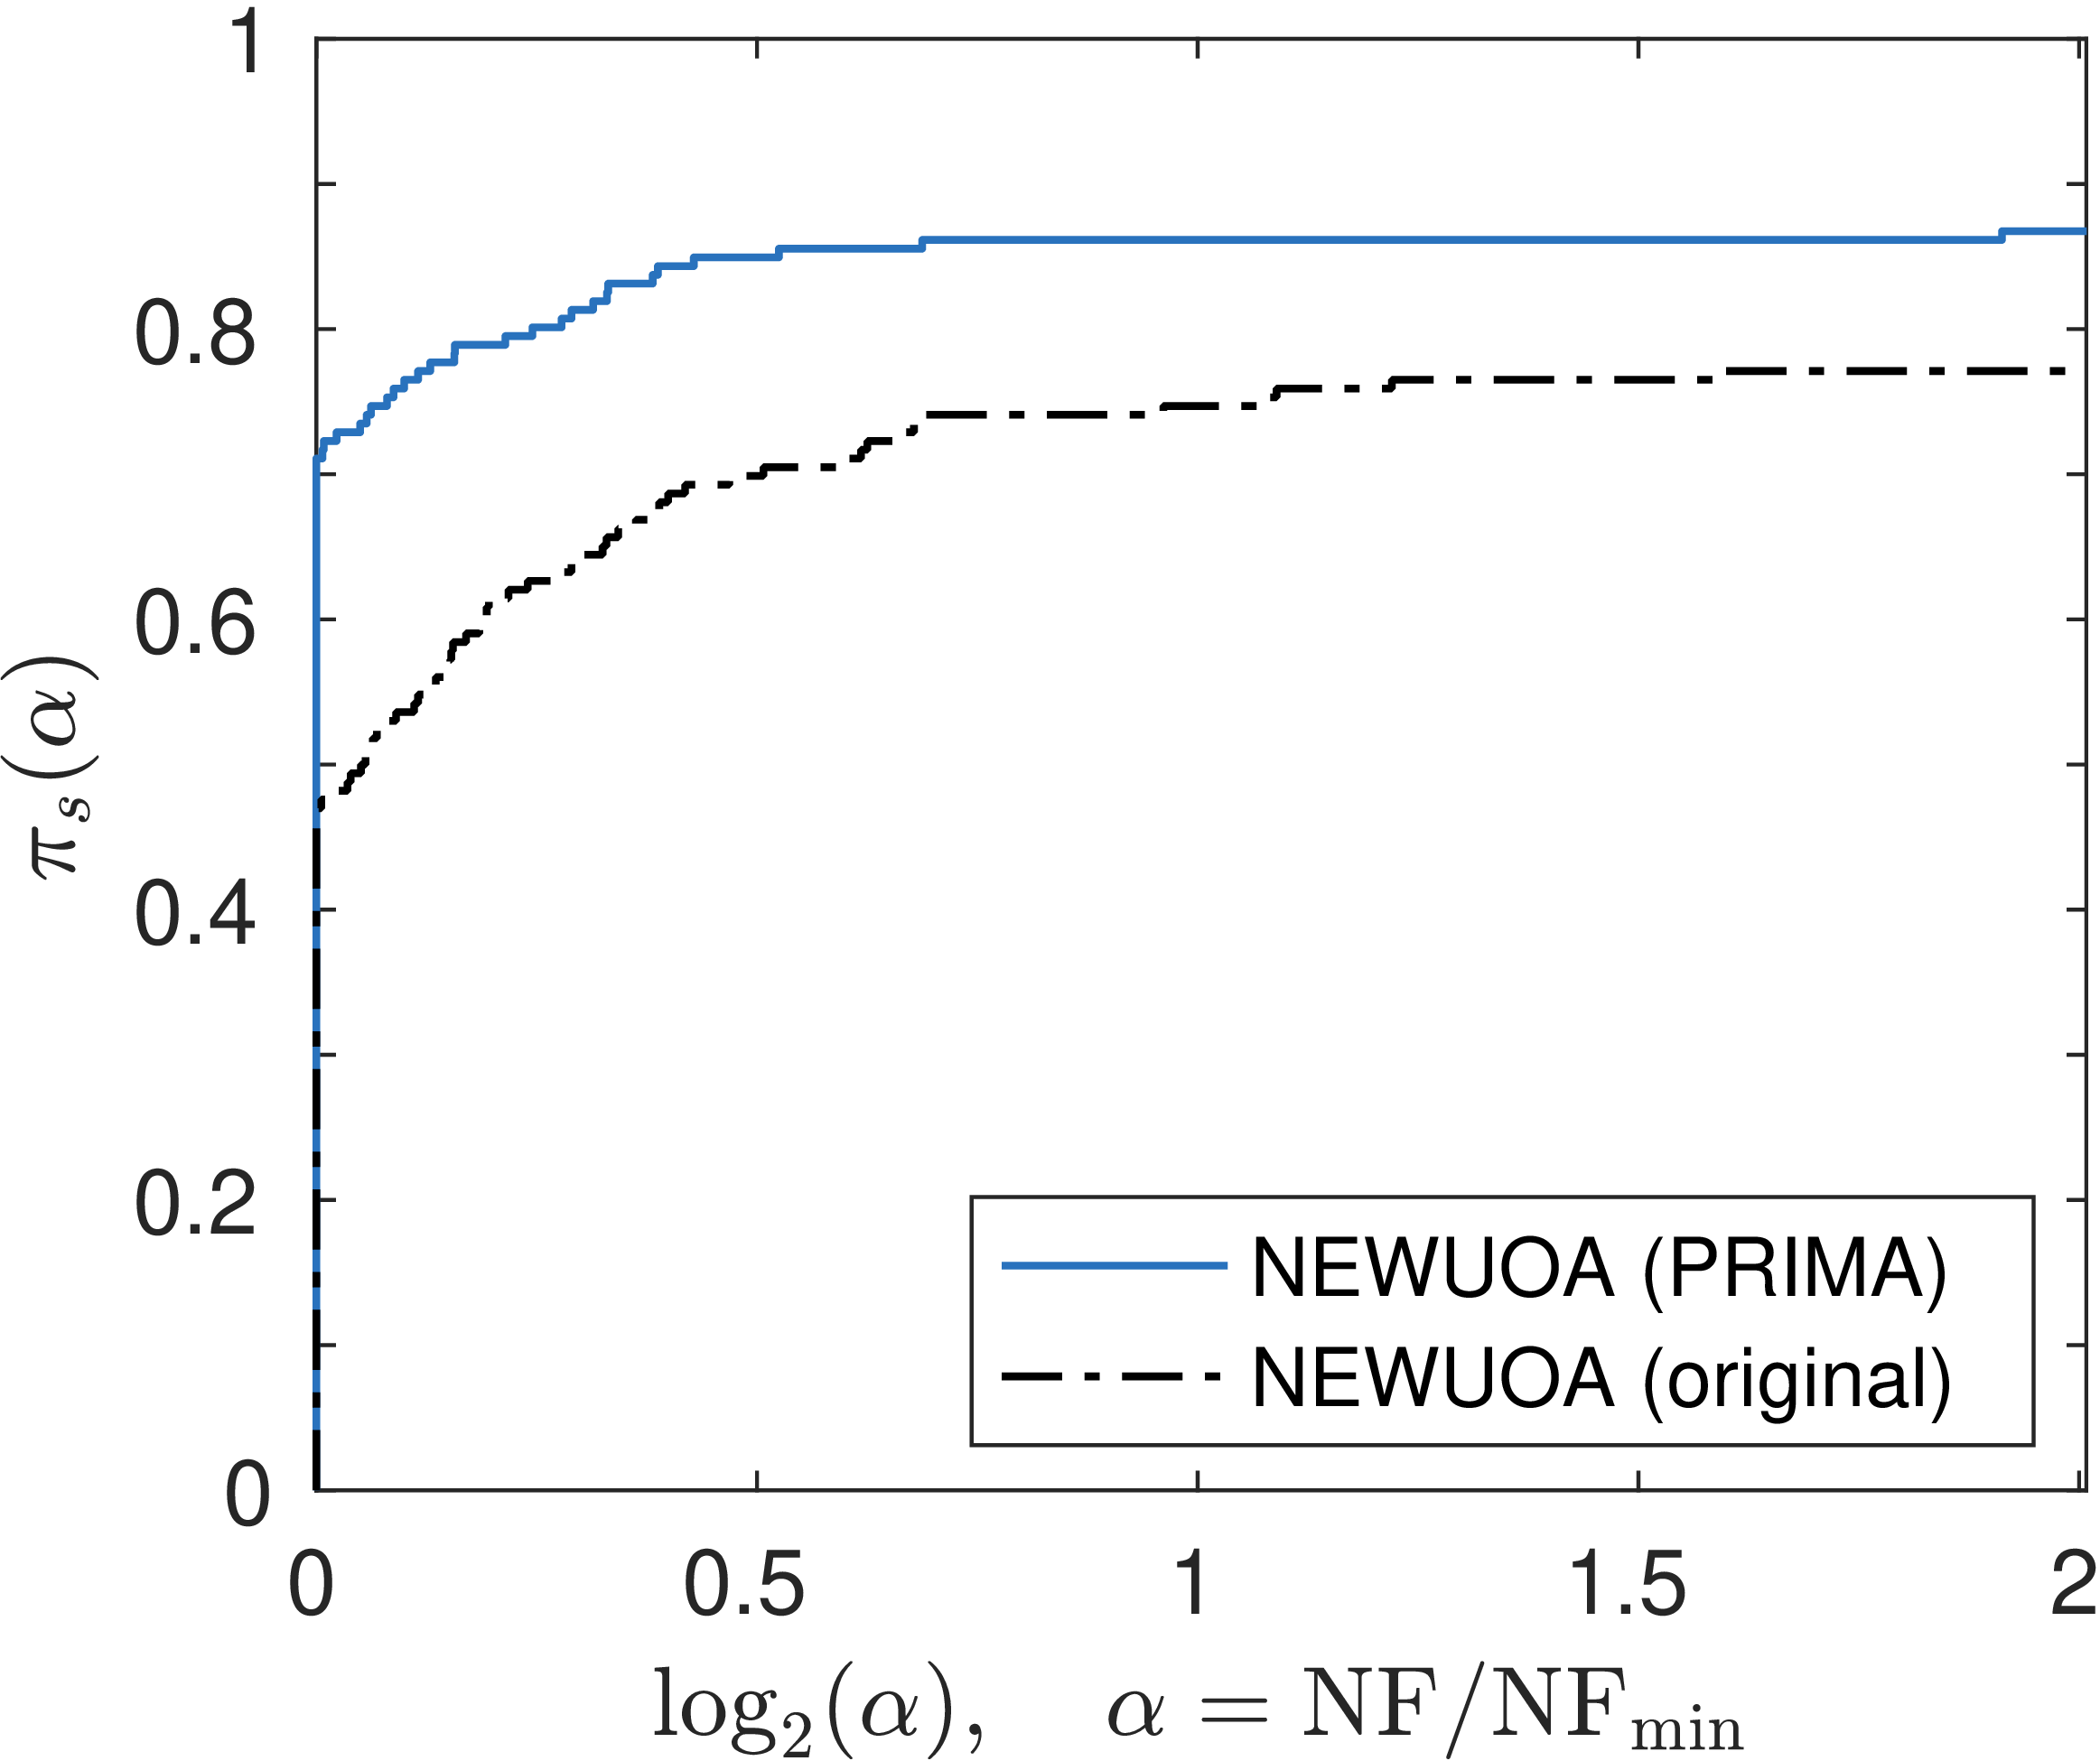
\includegraphics[width=0.5\textwidth]{prima_newuoa.png}
    \\[2ex]NEWUOA \\[1ex](unconstrained problems, at most 200 variables)
    \end{center}
\end{frame}

\begin{frame}
    \frametitle{The performance of PRIMA}
    \vspace{3ex}
    \begin{center}
    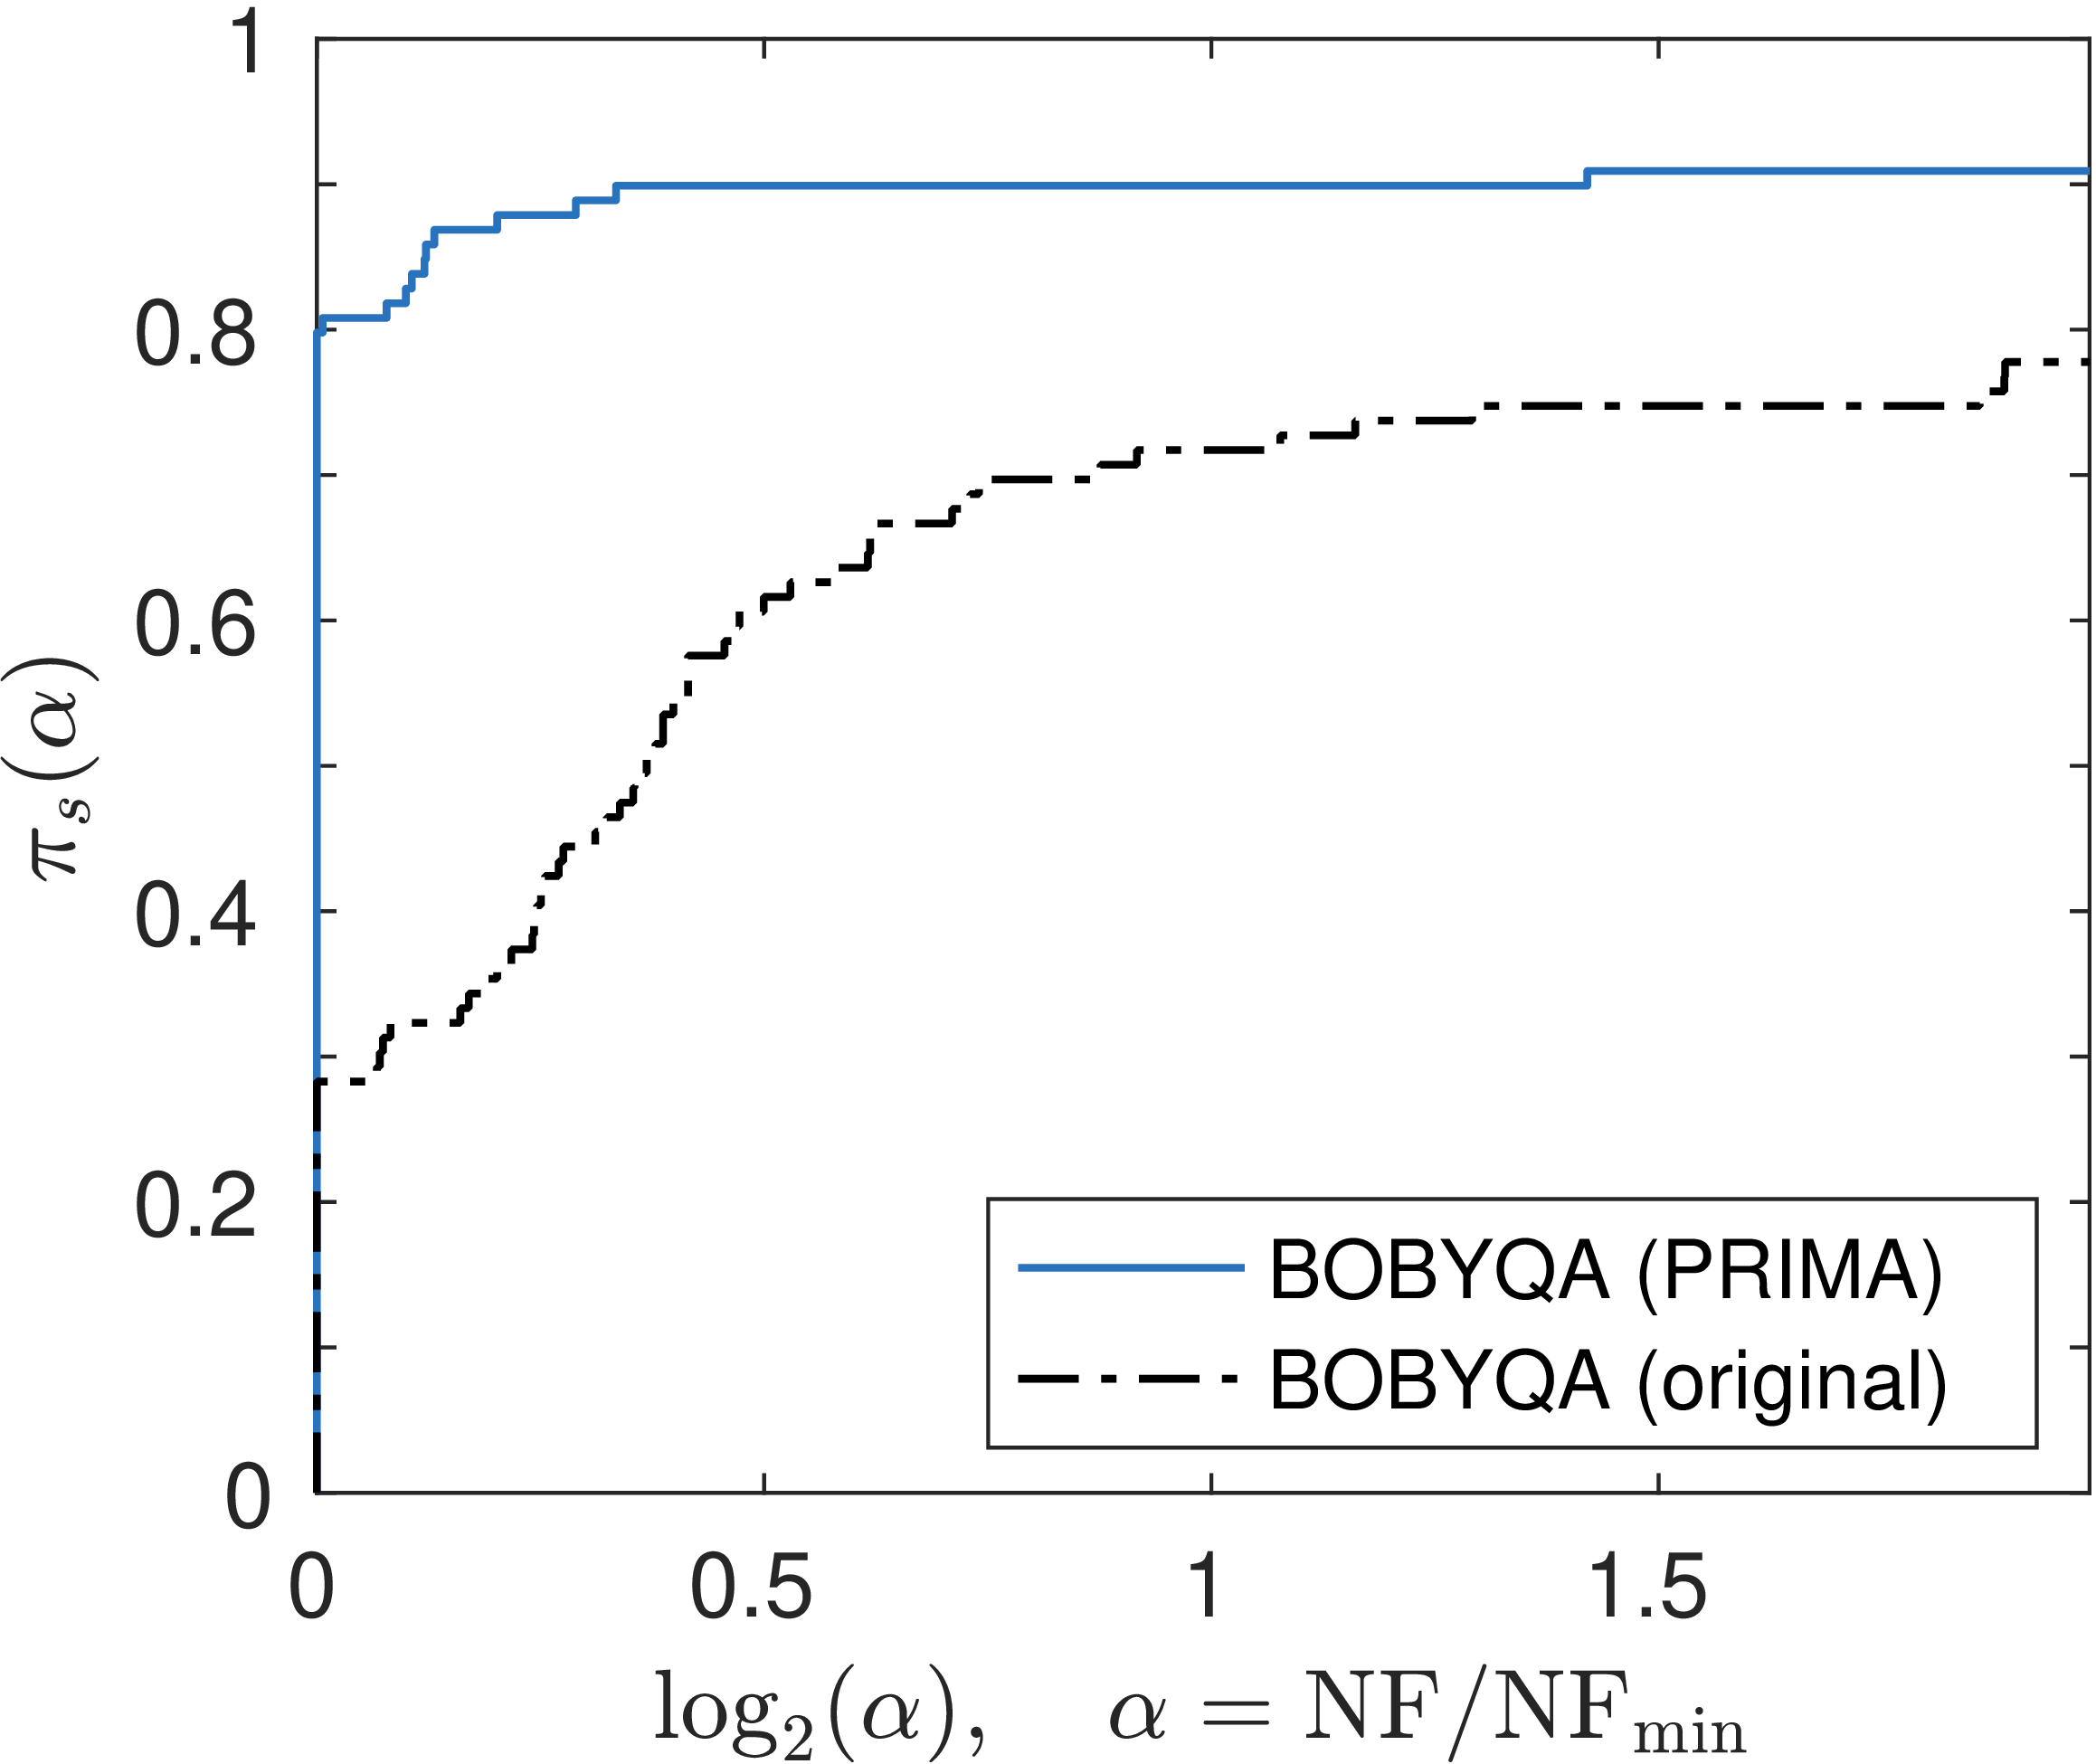
\includegraphics[width=0.5\textwidth]{prima_bobyqa.png}
    \\[2ex]BOBYQA \\[1ex](bound-constrained problems, at most 200 variables)
    \end{center}
\end{frame}

\begin{frame}
    \frametitle{The performance of PRIMA}
    \vspace{3ex}
    \begin{center}
    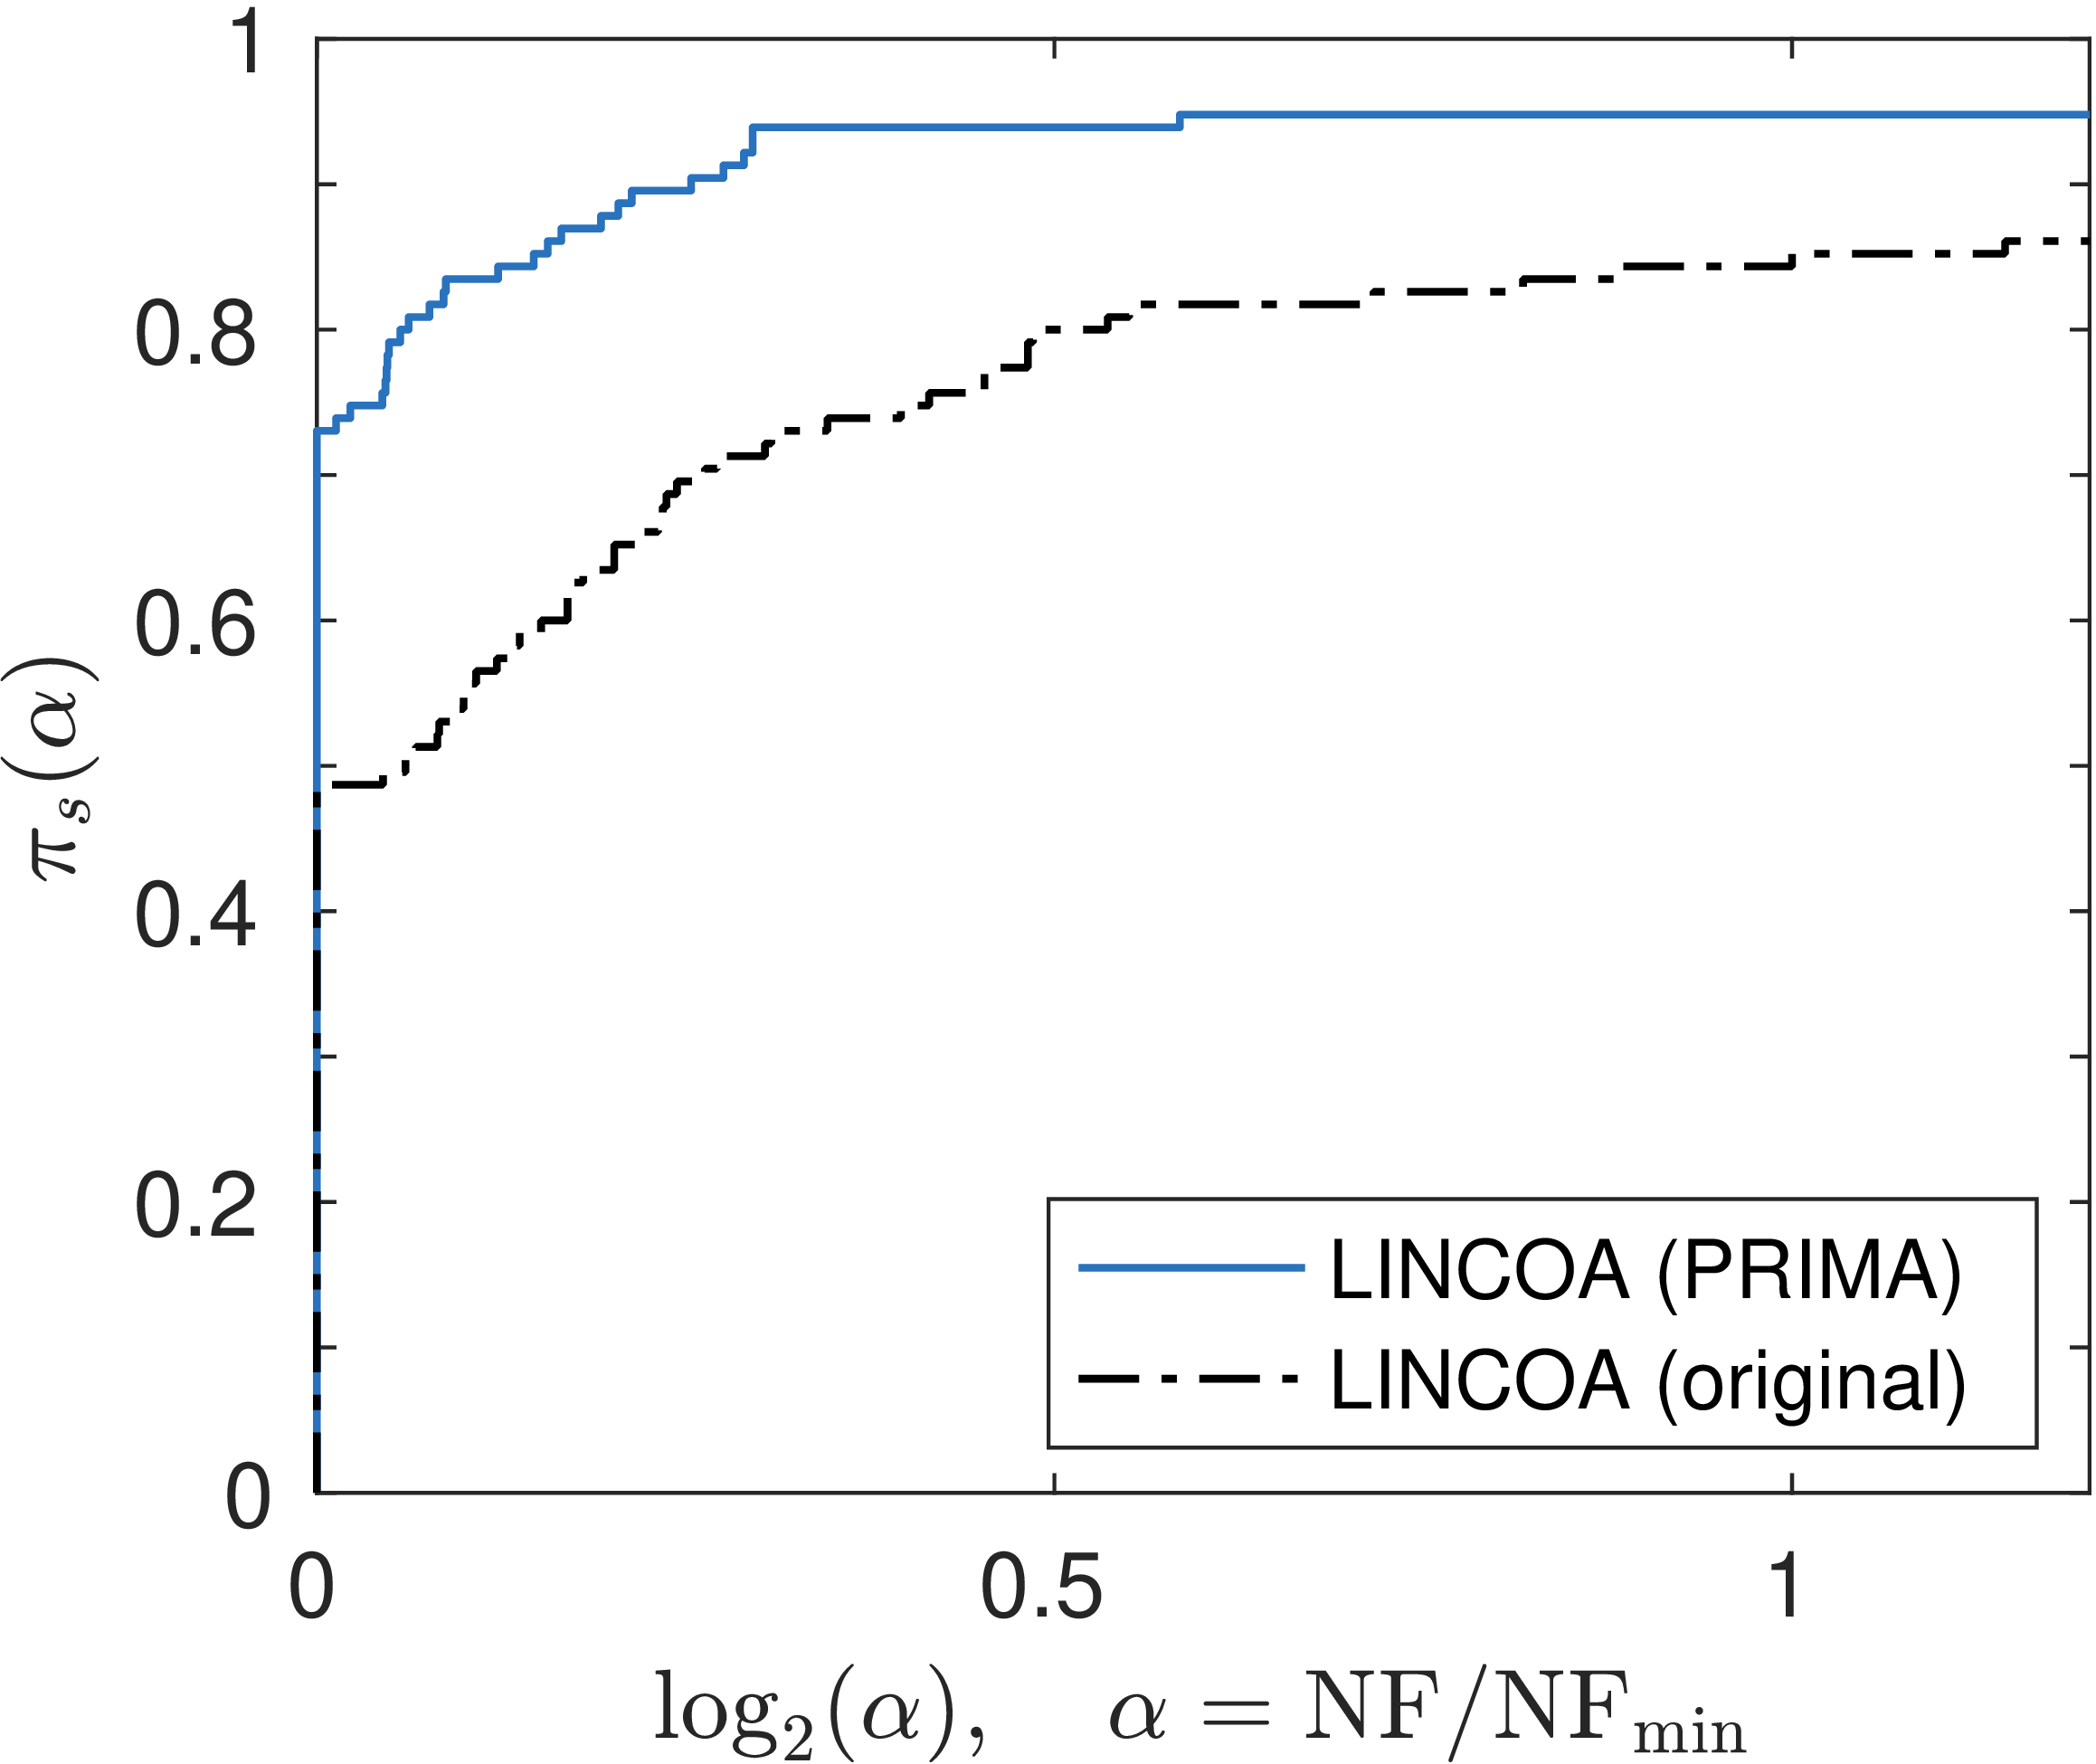
\includegraphics[width=0.5\textwidth]{prima_lincoa.png}
    \\[2ex]LINCOA \\[1ex](linearly constrained problems, at most 200 variables, 20,000 constraints)
    \end{center}
\end{frame}

\begin{frame}
    \frametitle{The performance of PRIMA}
    \vspace{3ex}
    \begin{center}
    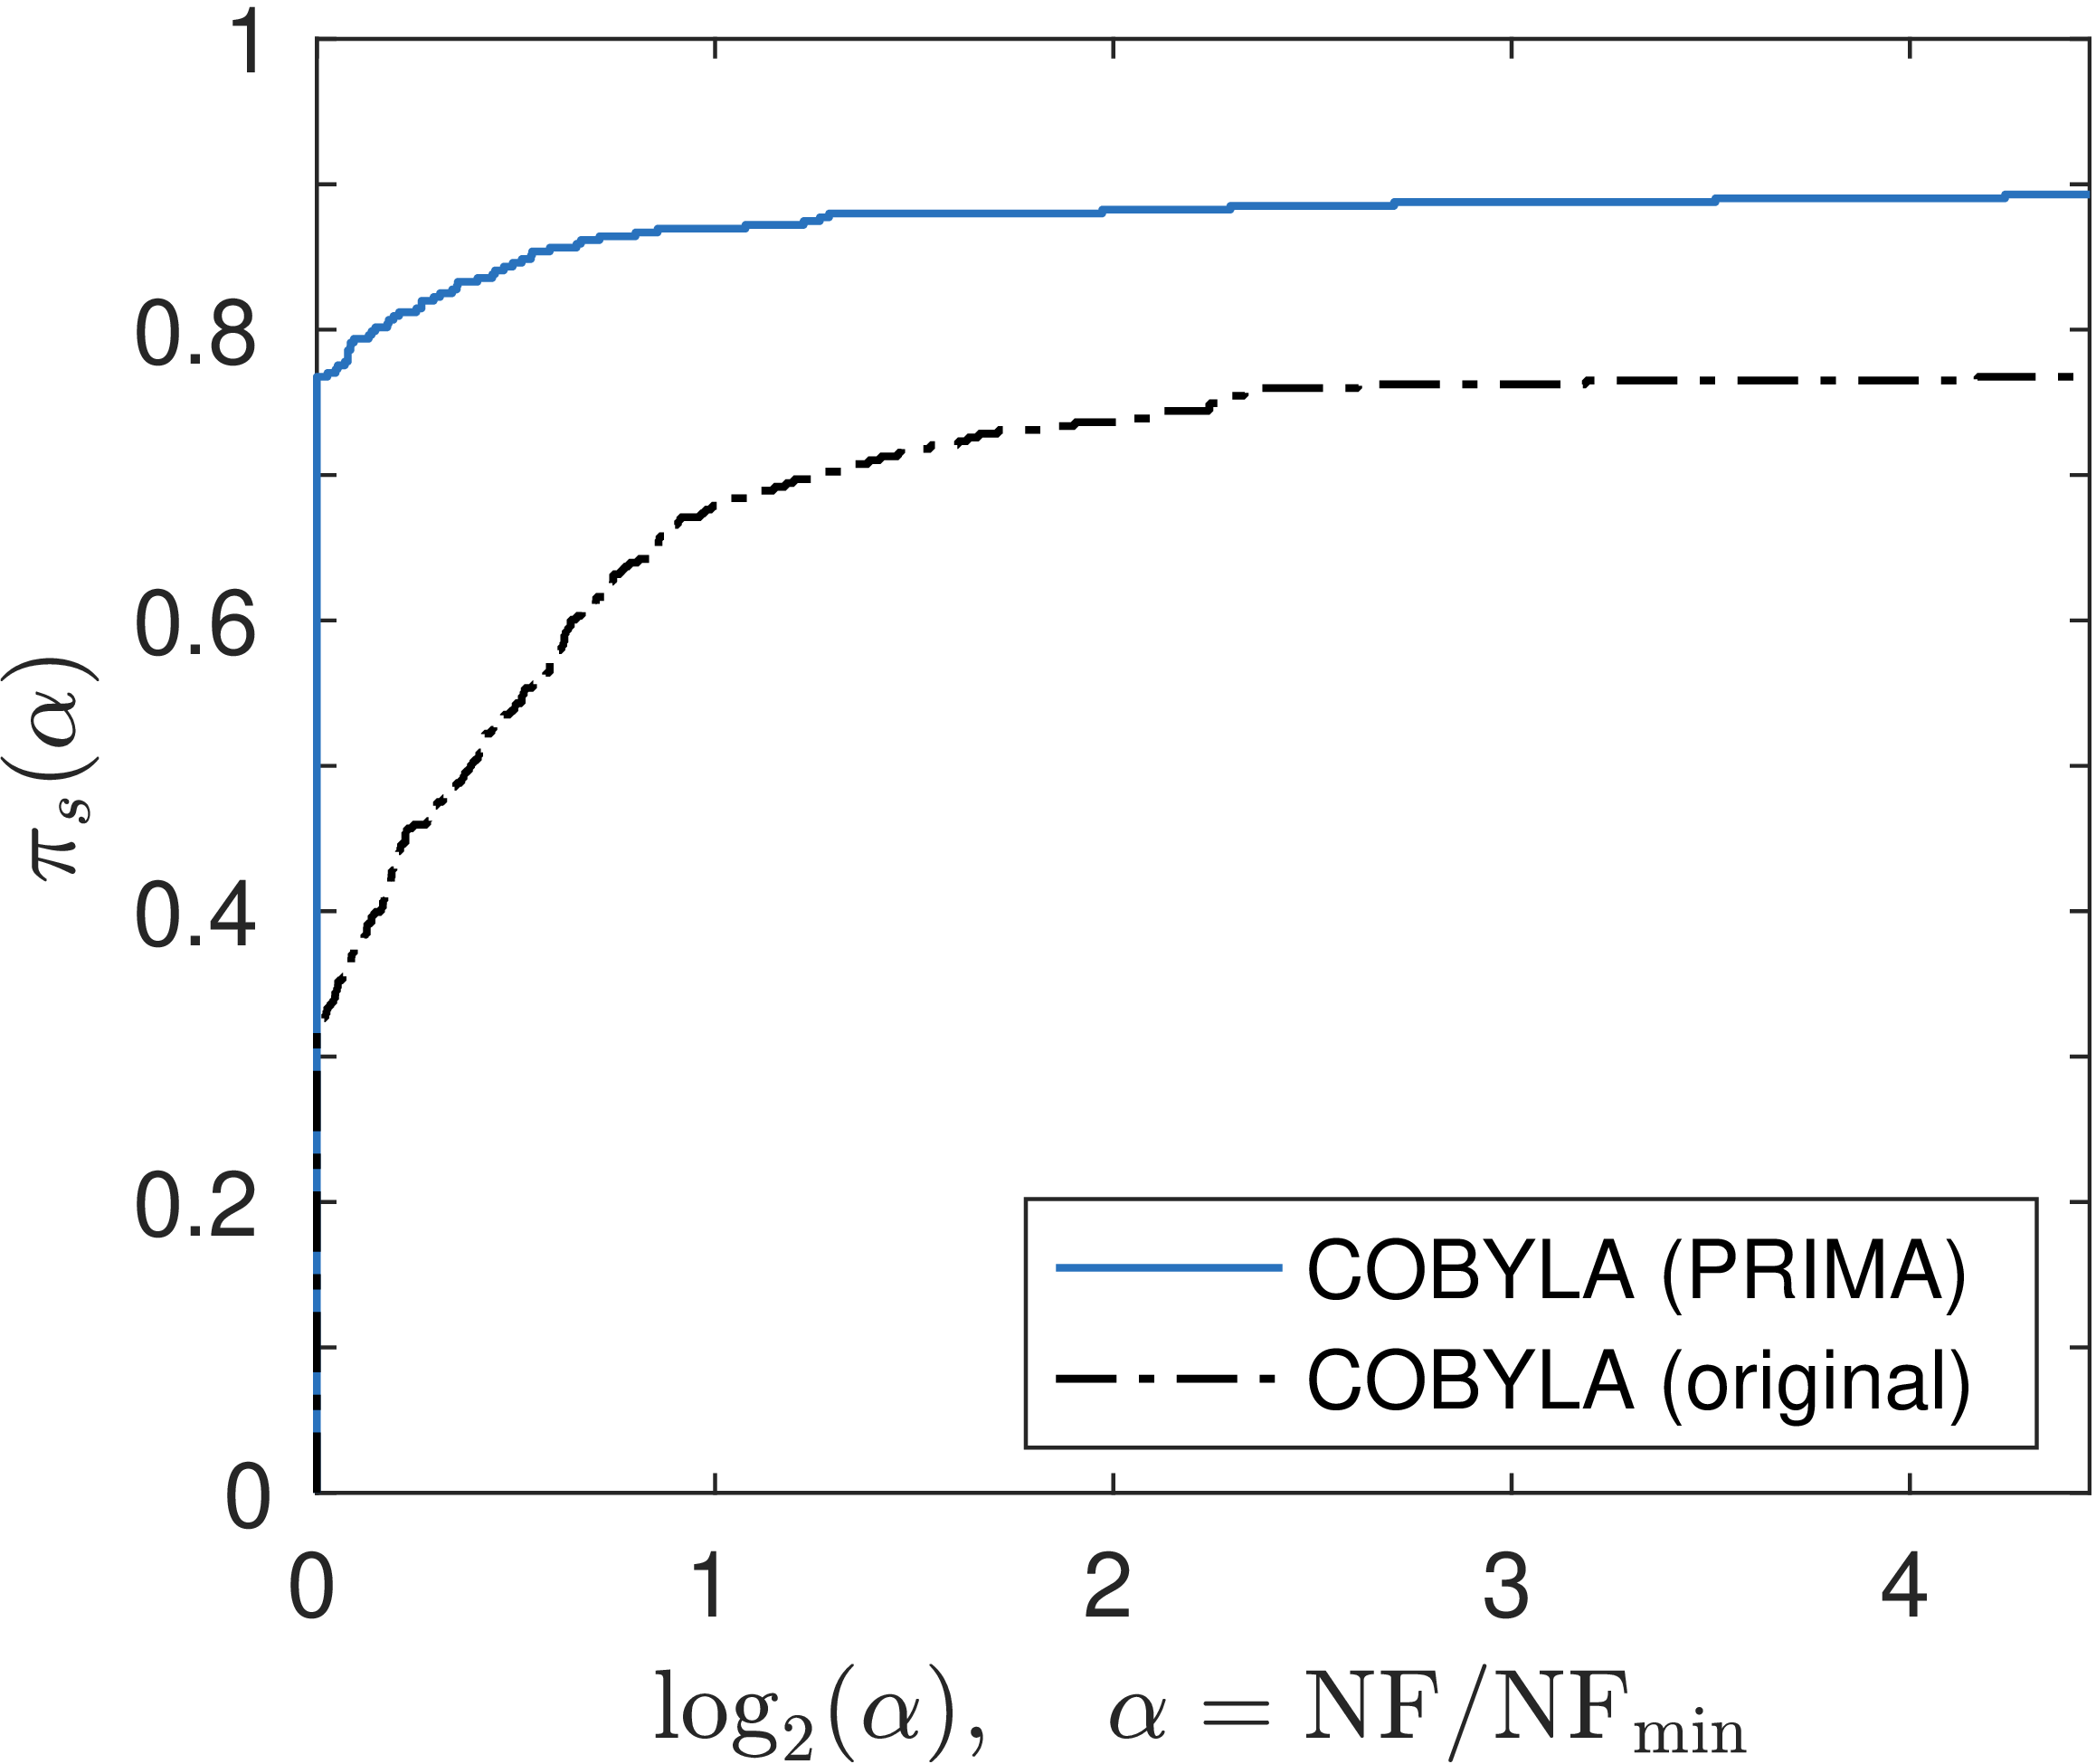
\includegraphics[width=0.5\textwidth]{prima_cobyla.png}
    \\[2ex]COBYLA \\[1ex]\mbox{\!\!(nonlinearly constrained problems, at most 100 variables,
    10,000 constraints)}
    \end{center}
\end{frame}


\begin{frame}
    \frametitle{How to ensure the improvements are not by luck?}
       Take COBYLA as an example. \\[1ex]
       The PRIMA implementation of COBYLA is tested on \blue{359} nonlinearly constrained CUTEst problems with
       \blue{at most 100 variables and 10,000 constraints}. \blue{Seven} tests are made.
        \vspace{1ex}
         \begin{enumerate}
             \item A plain test
                 \vspace{0.5ex}
             \item A test that permutes the variables randomly
                 \vspace{0.5ex}
             \item A test that perturbs the starting point randomly
                 \vspace{0.5ex}
             \item A test based on single-precision objective \& constraint values
                 \vspace{0.5ex}
             \item A test using only 5 significant digits of the objective~\&~constraints
                 \vspace{0.5ex}
             \item \mbox{A test contaminating the objective\! \&\! constraints by\!~deterministic\!~noise}%
                 \vspace{0.5ex}
             \item A test contaminating the objective \& constraints by random noise
         \end{enumerate}
\end{frame}


\begin{frame}
    \frametitle{How to ensure the improvements are not by luck?}
    \begin{center}
        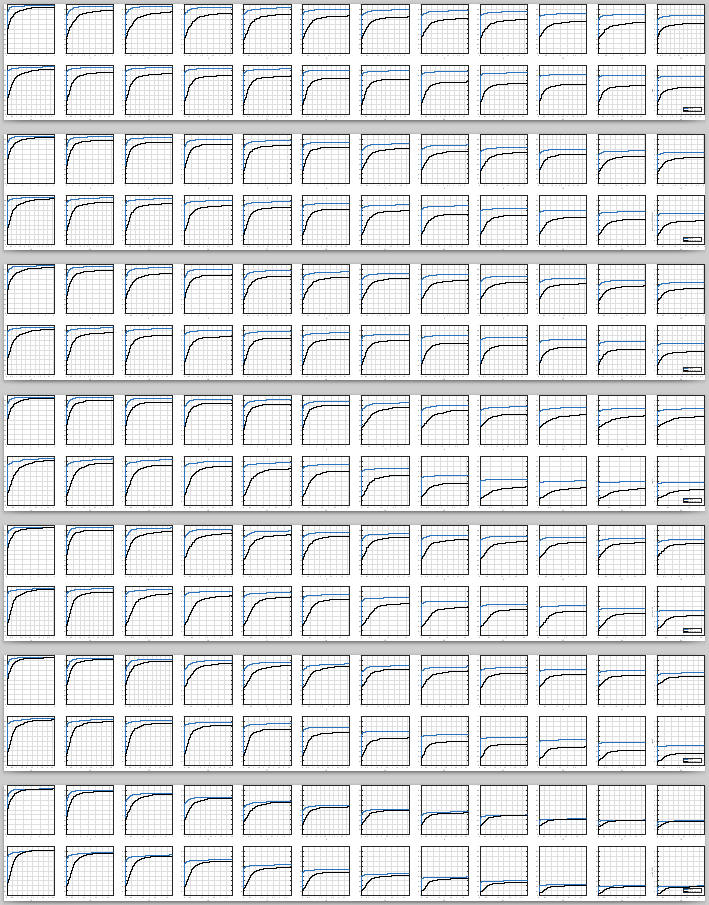
\includegraphics[width=0.45\textwidth]{cobyla_pp.png}
        \\[1ex]168 performance profiles of the new and old implementations of COBYLA
    \end{center}
\end{frame}

\begin{frame}
    \frametitle{A ``fun'' fact ...}

                 \vspace{1ex}
    \begin{itemize}
        \item
            Working on PRIMA, I have spotted \blue{a dozen of bugs} in reputable Fortran
            compilers and \blue{two bugs} in MATLAB.
                 \vspace{1ex}
        \item Each of them represents days of \red{bitter} debugging.
                 \vspace{1ex}
           %which finally led to the conclusion that it was not a problem in my code but a flaw in the Fortran compilers or in MATLAB.
        \item From an unusual angle, they reflect how intensive the coding is.
                 \vspace{1ex}
        \item The \red{bitterness} behind this fun fact is exactly why I work on PRIMA:
                 \vspace{0.6ex}
                 \begin{itemize}
                    \normalsize
                \item
                    {I hope all the \red{frustrations} that I have experienced will not
                    happen to any user of Powell's methods anymore.}
                 \vspace{0.6ex}
             \item \blue{I hope I am the last one} in the world to decode a maze of 244 GOTOs in 7939 lines of Fortran 77 code
--- I did this for three years and I do not want anyone else to do it again.
            \end{itemize}
    \end{itemize}
\end{frame}

\begin{frame}
    \frametitle{But it is not quite rewarding \red{in terms of career  and life} ...}

    \begin{itemize}
        \item You may write 3 good papers in 1 year, but not 1 good package in~3 years,~especially~if~you~start~with~a~nontrivial~Fortran~77~codebase.
            \vspace{1ex}
        \item \blue{Internet}: ``Writing software is a low-status academic~activity.''
            \vspace{1ex}
        \item \blue{Internet}: ``A general problem is that ... professors are usually rewarded for publications, not their software.''
           \vspace{1ex}
       \item \red{Comments on my grant proposal}: The PI's expertise seems in software development,
           but he \red{may not be a good mathematician}.
           \vspace{1ex}
       \item \blue{As a ``not-so-good mathematician''}, I much prefer spending my time on
           proofs, which are a lot easier and much more enjoyable for me.
    \vspace{1ex}
\item \red{Sometimes we do things that are not enjoyable but have to be done.}

    \vspace{1ex}
\item Teaser: \blue{Who translated Euclid's \textit{Elements}} to modern
    languages? \blue{You probably do not know (and do not care).}
    \end{itemize}

\end{frame}



\begin{frame}
  \frametitle{Concluding remarks}
    \begin{itemize}
        \item \red{Implementation of model-based DFO solvers is intrinsically hard}
            \vspace{0.5ex}
        \item \mbox{PRIMA provides the reference implementation of Powell's DFO~\!solvers\!}%
            \vspace{0.5ex}
        \item The modern Fortran version and a MATLAB interface is finished
            \vspace{0.5ex}
        \item \mbox{PRIMA will also be implemented in MATLAB, Python, Julia, R, C\texttt{++}}
            \vspace{0.5ex}
        \item PRIMA fixes issues in the original Fortran 77 code
            \vspace{0.5ex}
        \item PRIMA is tested extensively to ensure its correctness \& robustness%
            \vspace{0.5ex}
        \item PRIMA outperforms the original implementation of the solvers
    \end{itemize}

%  \vspace{-2ex}

    \begin{center}
    \qrcode[height=0.15\textwidth]{http://www.libprima.net}
    \\[1.6ex]\href{http://www.libprima.net}{\blue{\texttt{libprima.net}}}
    \end{center}
    %\begin{columns}[T]
    %    %\begin{column}{0.3\textwidth}
    %    %    \begin{center}
    %    %    \qrcode[height=0.5\textwidth]{https://github.com/newuoas/newuoas}
    %    %    \\[2ex]\href{https://github.com/newuoas/newuoas}{\blue{NEWUOAs}}
    %    %    \end{center}
    %    %\end{column}
    %    \begin{column}{0.4\textwidth}
    %        \begin{center}
    %        \qrcode[height=0.5\textwidth]{http://www.libprima.net}
    %        \\[2ex]\href{http://www.libprima.net}{\blue{PRIMA}}
    %        \end{center}
    %    \end{column}
    %    \begin{column}{0.4\textwidth}
    %        \begin{center}
    %            \qrcode[height=0.5\textwidth]{https://github.com/equipez/matcutest}
    %            \\[2ex]\href{https://github.com/equipez/matcutest}{\blue{MatCUTEst}}
    %        \end{center}
    %    \end{column}
    %\end{columns}

  %\vspace{1ex}

    \begin{center}
      { \Large{\textcolor{blue}{Thank you!}}}
%      \\[1ex]\url{zaikun.zhang@polyu.edu.hk}
    \end{center}


\end{frame}
\end{document}

%\begin{frame}
%    \frametitle{What kind of code do we write?}

%    \vspace{3ex}


%    \begin{enumerate}
%        \item Dirty, secret research code
%            \vspace{1ex}
%        \item Clean, public research code
%            \vspace{1ex}
%        \item Open-source software package
%            \vspace{1ex}
%        \item \red{Tested} open-source software package
%            \vspace{1ex}
%        \item Industrial software package
%    \end{enumerate}

%\end{frame}

%\begin{frame}
%    \frametitle{``Research software code is likely to remain a tangled mess''}
%    \vspace{3ex}
%    \begin{mybox}
%        \textnormal{Research software (i.e., software written to support research in engineering or the
%            sciences) is usually a tangled mess of spaghetti code that only the author knows how to use.
%            Very occasionally I encounter well organized research software that can be used without
%            having an email conversation with the author (who has invariably spent years iterating
%            through many versions).
%        }
%    \end{mybox}
%    \begin{flushright}
%     --- \url{https://bit.ly/3oMzqQw}
%    \end{flushright}
%    ~\\[1ex]\nb: This comment is copied from a blog. It is not by or from me.
%\end{frame}

%\begin{frame}
%    \frametitle{What is the reason?}

%    \vspace{3ex}
%    The following comments are \blue{copied} from the aforementioned blog and online discussions about it. \\[2ex]

%    \begin{enumerate}
%        \item Writing software is a low status academic activity.
%            \vspace{1ex}
%        \item  A general problem is that graduate students, post-docs, and professors are usually
%            rewarded for publications, not their software.
%            \vspace{1ex}
%        %\item Many of those writing software know very little about how to do it, and don't have daily contact with people who do.
%        \item A common misconception is that because the mathematics is correct, the software must
%        be correct (completely ignoring the possibility of silly coding mistakes, which everybody
%        makes). Commercial software has the benefit of user feedback, for detecting some incorrect
%        failures. Research software may only ever have one user.
%    \end{enumerate}
%\end{frame}

%\begin{frame}
%    \frametitle{What is the consequence?}
%    \begin{center}
%    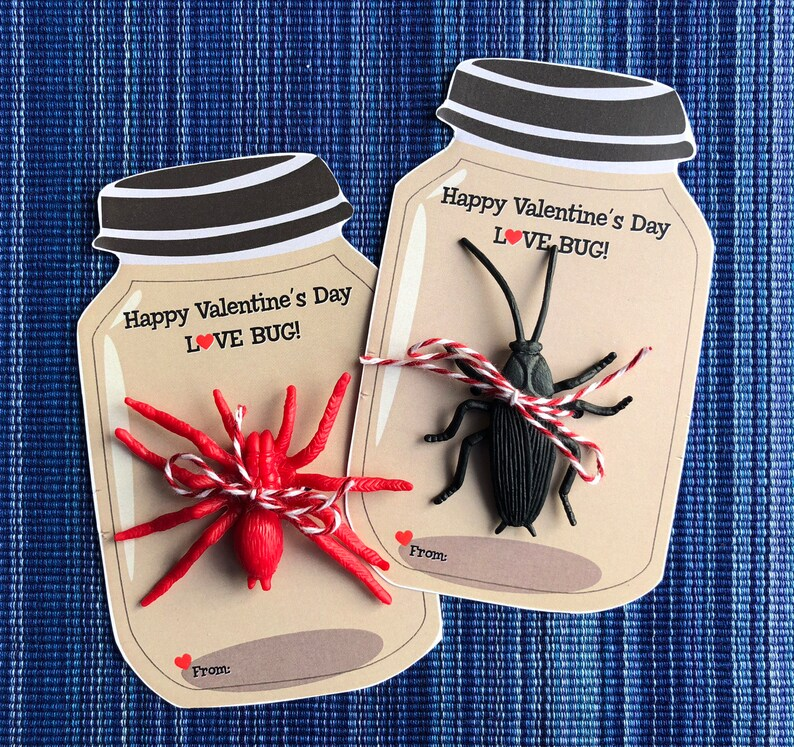
\includegraphics[width=0.5\textwidth]{exchange_bugs.jpg}
%    \\[2ex] ``Researchers used to exchange experimental data and now they exchange software bugs.''
%    \end{center}

%\end{frame}



%\begin{frame}
%    \frametitle{Why optimize a function without using derivatives?}
%    \vspace{-2ex}
%    \begin{center}
%    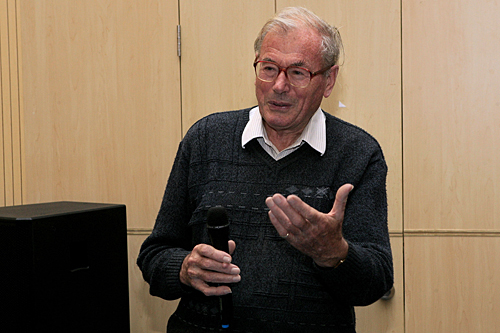
\includegraphics[width=0.5\textwidth]{Powell.jpg}
%    \end{center}
%    \begin{beamerboxesrounded}[width=12.08cm,shadow=true]{}
%      \small
%      I started to write computer programs in {Fortran}
%        at \textcolor{blue}{Harwell in 1962}.
%        ... after moving \textcolor{blue}{to Cambridge in 1976} ...  I became a consultant
%        for \red{IMSL}. One product they received from me was the
%        \texttt{\textcolor{blue}{TOLMIN}} package
%    for optimization ... which requires first derivatives ...
%    \textcolor{blue}{Their
%    customers, however,
%    prefer methods that are without derivatives}, so IMSL forced my
%    software
%    to employ \textcolor{blue}{difference approximations} ...
%    \textcolor{red}{I was not happy} ... Thus there was strong motivation to try to
%    construct some better algorithms.
%    \end{beamerboxesrounded}
%    \vspace{-0.3ex}
%    \begin{flushright}
%        --- {M. J. D. Powell}
%    \vspace{0.3ex}
%        \small{\\A view of algorithms for optimization without
%        derivatives, 2007, Hong Kong}
%    \end{flushright}
%\end{frame}

%\begin{frame}
%    \frametitle{\newuoas}
%    \begin{center}
%    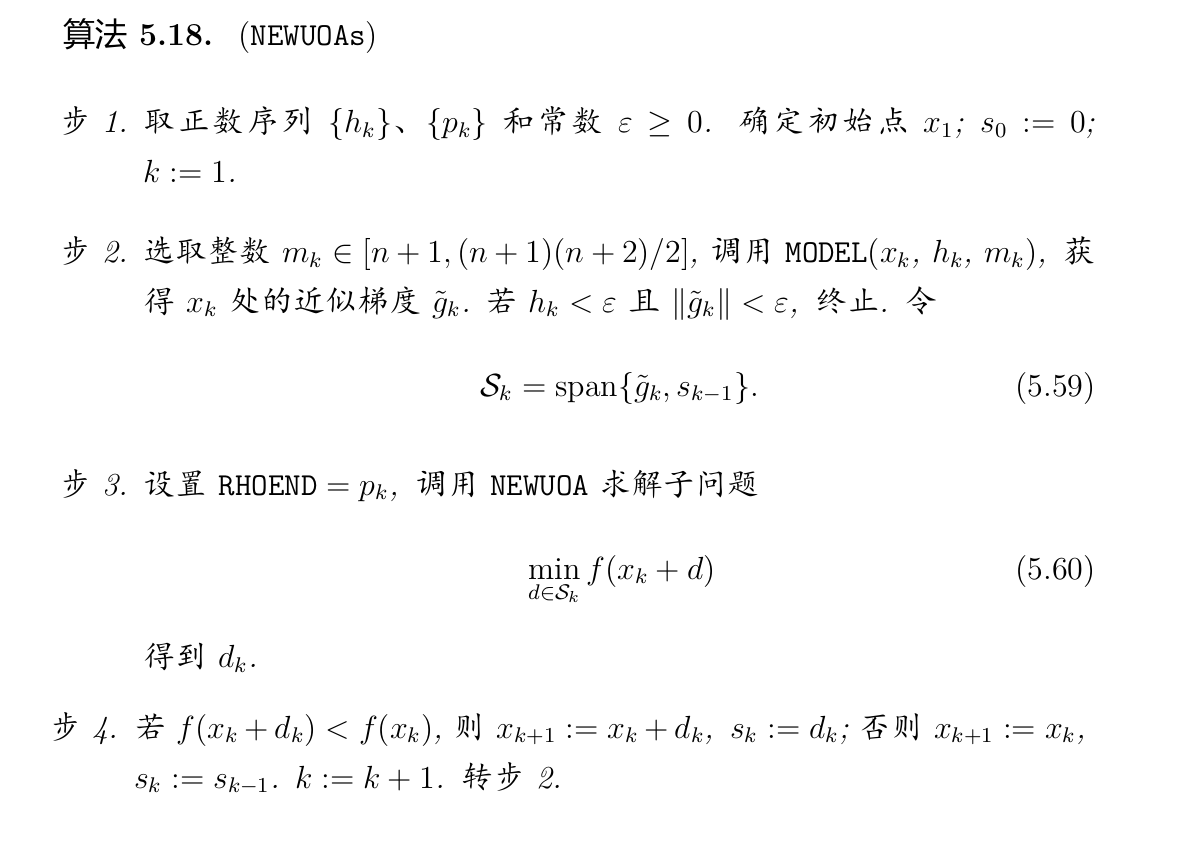
\includegraphics[width=0.86\textwidth]{newuoas.png}
%    \end{center}
%    \vspace{-2ex}
%    \begin{center}
%        \newuoas (\blue{screen-shot} taken from Sec.~5.3.3 of my Ph.D. thesis, 2012)
%    \end{center}
%\end{frame}

%\begin{frame}
%    \frametitle{More information on \newuoas}

%    \begin{itemize}
%        \item \newuoas is fully described in Sec.~5.3 of\\[0.5ex]
%            \small{Zhang, \textcolor{blue}{\textit{On Derivative-Free Optimization Methods}} (无导数优化方法的研究), Ph.D. thesis, Chinese Academy of Sciences, Beijing, 2012}
%            \vspace{1ex}
%        \item A \blue{general framework} for subspace methods is given in Sec.~5.3.1 of the thesis.
%            \vspace{1ex}
%        \item \blue{Implementation details} of \newuoas are presented in Sec.~5.3.5 of the thesis.
%            \vspace{1ex}
%        \item The \blue{MATLAB implementation of \newuoas} is available at
%            \begin{center}
%                \href{https://github.com/newuoas/newuoas}{{\url{https://github.com/newuoas/newuoas}}}\;.
%            \end{center}
%            \vspace{1ex}
%        \item \newuoas is included as a DFO solver in the \blue{open-source package \texttt{cm3}} at
%            \begin{center}
%                \href{https://github.com/modula3/cm3}{{\url{https://github.com/modula3/cm3}}}
%            \end{center}
%            under \href{https://github.com/modula3/cm3/blob/master/caltech-other/newuoa/src/NewUOAs.m3}
%            {\blue{\texttt{caltech-other/newuoa/src/NewUOAs.m3}}}\;.
%    \end{itemize}
%    \vspace{-2ex}
%    \begin{columns}[T]
%        \begin{column}{0.4\textwidth}
%            \begin{center}
%            \qrcode[height=0.375\textwidth]{https://github.com/newuoas/newuoas}
%            \\[1ex]\href{https://github.com/newuoas/newuoas}{\blue{\texttt{github.com/newuoas}}}
%            \end{center}
%        \end{column}
%        \begin{column}{0.4\textwidth}
%            \begin{center}
%            \qrcode[height=0.375\textwidth]{https://github.com/modula3/cm3/blob/master/caltech-other/newuoa/src/NewUOAs.m3}
%            \\[1ex]\href{https://github.com/modula3/cm3/blob/master/caltech-other/newuoa/src/NewUOAs.m3}
%            {\blue{\texttt{github.com/cm3}}}
%            \end{center}
%        \end{column}
%    \end{columns}
%\end{frame}


%\begin{frame}
%    \frametitle{ \newuoas solving some 2000-dimensional Problems}
%\begin{table}
%    \centering
%    %\caption{The Performance of \newuoas on some 2000-dimensional Problems}
%    \label{tab:newuoas2000}
%    \begin{tabular}{lllll}
%        \toprule
%        &  $f_{\textnormal{start}}$& $f_{\textnormal{best}}$& $\#f$ &CPU (s)\\
%\midrule
%ARWHEAD&   5.997000E$+$03&  0.000000E$+$00& 16095&  6.42 \\
%BRYBND&    7.200000E$+$04&  6.486038E$-$09& 50000&  26.09 \\
%DIXMAANE&  1.471453E$+$04&  1.000000E$+$00& 36264&  21.12 \\
%DIXMAANF&  2.734976E$+$04&  1.000000E$+$00& 36384&  31.07 \\
%DIXMAANG&  5.069653E$+$04&  1.000000E$+$00& 36393&  22.72 \\
%DQRTIC&    6.376035E$+$15&  1.214880E$-$38& 40854&  14.70 \\
%GENHUMPS&  5.122260E$+$07&  1.624799E$-$26& 36467&  23.54 \\
%LIARWHD&   1.170000E$+$06&  2.428807E$-$24& 16208&  6.73 \\
%POWER&     2.668667E$+$09&  1.423292E$-$11& 20130&  19.19 \\
%SPARSQUR&  5.627812E$+$05&  6.381755E$-$30& 16209&  9.87 \\
%\bottomrule
%    \end{tabular}
%\end{table}
%\vspace{1ex}
%N.B.: These results are from 2012. In 2023, we can do \blue{much better}.
%\end{frame}
